%% ----------------------------------------------------------------
%% Thesis.tex -- MAIN FILE (the one that you compile with LaTeX)
%% ---------------------------------------------------------------- 

% Set up the document
\documentclass[a4paper, 11pt, oneside]{Thesis}  % Use the "Thesis" style, based on the ECS Thesis style by Steve Gunn
\graphicspath{Figures/}  % Location of the graphics files (set up for graphics to be in PDF format)

% Include any extra LaTeX packages required
\usepackage[square, numbers, comma, sort&compress]{natbib}  % Use the "Natbib" style for the references in the Bibliography
\usepackage{verbatim}  % Needed for the "comment" environment to make LaTeX comments
\usepackage{vector}  % Allows "\bvec{}" and "\buvec{}" for "blackboard" style bold vectors in maths
\hypersetup{urlcolor=blue, colorlinks=true}  % Colours hyperlinks in blue, but this can be distracting if there are many links.
\usepackage{amsmath}
\usepackage{blkarray}
\usepackage{float}
\usepackage{epstopdf}

% LaTeXDraw includes
\usepackage[usenames,dvipsnames]{pstricks}
\usepackage{epsfig}
\usepackage{pst-grad} % For gradients
\usepackage{pst-plot} % For axes
\usepackage[space]{grffile} % For spaces in paths
\usepackage{etoolbox} % For spaces in paths
\usepackage{multirow}
\usepackage{pdfpages}

\newcommand{\norm}[1]{\left\lVert#1\right\rVert}
\newcommand{\brk}{\vspace*{0.18in}}

%% ----------------------------------------------------------------
\begin{document}
\frontmatter      % Begin Roman style (i, ii, iii, iv...) page numbering


% Set up the Title Page
\title{}
\title  {Efficient Factor Graph Fusion for Multi-robot Mapping}
\authors  {\texorpdfstring
          {\href{nrkumar93@gmail.com}{Ramkumar Natarajan}}
          {Ramkumar Natarajan}
          }
%\addresses  {\groupname\\\deptname\\\univname}  % Do not change this here, instead these must be set in the "Thesis.cls" file, please look through it instead
%\date       {\today}
%\subject    {}
%\keywords   {}

%% FIRST OF ALL:
% If you are using X-based Emacs to read this file, please switch on
% Syntax Highlighting by typing:
%    ALT-X  font-lock-mode   (or META-X on X-Terminals)
%
% That should make these comments nice and red so they can be easily
% distinguished from the actual code. 
% =======================================================================

% This is a template for  Masters' Theses at WPI.
% It complies (more or less) to the standards given by the Library 
% (as of February 1999)
%
% Feel free to use this file, but I give no guarantee for its compliance
% to standards (meaning I won't pay for the paper if the library rejects it :))
%
%
% The lengths (textheight, width etc.) are fine-tuned for ps1, ps2, and ps3, 
% but seem to be somewhat dependent on the machine you are using to compile, 
% the date, time, moon phase, the weather, and other quantum effects.
% You may have to change \oddsidemargin a little, but it's about 98% correct.
%
% Also, the spacing is correct (doublespacing with footnotes correctly
% singlespaced). Curiously, the font size is not specified in the
% regulations. So feel free to change it, but the majority of theses
% that I have seen is written in 12 point font.
% 
% As for the inclusion of graphics, I recommend the methods specified
% in ``latexguide.ps'' off the CS-GSO Website. You can use other
% methods including copy and paste with a photocopier, but I think
% using the graphicx package is the easiest.
%
% Have fun and good luck with the thesis.
%
%
%  Andreas Koeller (koeller@wpi.edu)
%
%
%

% The preamble
%
%
% 12 point font, and your thesis is a ``report'' to LaTeX
%\documentclass[12pt]{report}
%
%% this enables correct linespacing and graphics inclusion via 
%%``\includegraphics''
%\usepackage{setspace}
%\usepackage{graphicx}
%
%
%% leave 1.5in margin to the left and 1in margin to the other
%% sides. Don't print page number in the margin (but rather above it)
%\setlength{\textheight}{8.63in}
%\setlength{\textwidth}{5.9in}
%\setlength{\topmargin}{-0.2in}
%\setlength{\oddsidemargin}{0.3in}
%\setlength{\evensidemargin}{0.3in}
%\setlength{\headsep}{0.0in}
%
%% Start to write
%\begin{document}

% First things first: The Titlepage
% This is the recommended format by the library
%


% Define \brk as a command for leaving a little vertical space. Makes
% the titlepage easier to read - normally, this is NOT GOOD LATEX
% STYLE!!!
%
\newcommand{\brk}{\vspace*{0.18in}}

% No page number on the title page
\thispagestyle{empty}

% Center the whole title page
\begin{center}

\brk

% Large font and bold face for the headline. Try to keep it at one or
% two lines. Headlines over two lines will mess up the spacing, and you have to
% manually finetune it. Note that the line break in the SOURCE CODE
% does not affect the line breaking in the output file. If you want
% hardcoded line breaks, you have to mark them with a double backslash (\\)

%   {\large 
%	\textbf{
%	Efficient Factor Graph Fusion
%	for Multi-robot Mapping
%	}
%   }
\title  {Efficient Factor Graph Fusion \\ for Multi-robot Mapping}
\maketitle

\brk
by

\brk
% insert your name here. 
Ramkumar Natarajan


% All this is constant:
\brk\brk
A Thesis

\brk
Submitted to the Faculty

\brk
of the 

\brk
WORCESTER POLYTECHNIC INSTITUTE
	
\brk
In partial fulfillment of the requirements for the

\brk
Degree of Master of Science

\brk
in

\brk
Robotics Engineering

\brk
by

% This is how LaTeX draws lines :) It's where your signature goes.
\brk\brk
\rule{3in}{1.2pt}

% Adjust this to your preferred month and year
\brk
May 2017

\end{center}

	
\vfill
APPROVED:

\vspace{0.5in}
\rule{3in}{0.8pt}

% Change this to your favorite CS professor.
Professor Michael A. Gennert, Thesis Advisor

\vspace{0.5in}
\rule{3in}{0.8pt}

% This is also constant :)
Professor William R. Michalson, Thesis Committee Member	

\vspace{0.5in}
\rule{3in}{0.8pt}

% This is also constant :)
Professor Eugene Eberbach, Thesis Committee Member	

% end of titlepage
%\newpage
%
%% This is the command for doublespacing when you use the setspace
%% package
%% Please do NOT use \baselinestretch, this will mess up everything,
%% cause earthquakes, tornados and lots of questions for me...
%% If you need a singlespaced paragraph (BAD STYLE!!!), use
%% \singlespacing or \onehalfspacing and enclose it together with the
%% paragraph in braces {\singlespacing This is my text... blah blah blah}
%%
%\doublespacing
%
%% Now you can start to be creative.
%% First, you need an abstract.
%% Fortunately, LaTeX has thought of that, so it's very easy:
%%
%\begin{abstract}
%This paper is the most important paper I have ever written. Therefore,
%everyone should read it, like it, and recommend it to all his friends.
%\end{abstract}
%
%% From here on, we need Roman page numbers according to the library
%% regulations. So let's assign those.
%
%\pagenumbering{roman} % or {Roman} if you like them capitalized
%
%% The next thing is the Preface (``Acknowledgements'').
%% No standard environment for that, so we'll format it by hand.
%%
%\begin{center}
%	\textbf{Acknowledgements}
%\end{center}
%
%	I would like to express my gratitude to my advisor who made
%	sure the thesis has at least 120 pages, 200 pictures and lots
%	of formulae and thus made me master \LaTeX{} like my native
%	language.
%
%        My thanks are also due to my reader... who has read the thesis
%        in the two days that I gave him since it wasn't done until two
%        days before due date.
%
%	Thanks also to ... lots of friends, the fact that a week has
%	seven days instead of only five as I had always thought, and
%	the fact that I own a key to the building so I can work at four
%	in the morning whenever I feel like it. That is, all the time.
%
%% P.S. You don't have to add me to the acknowledgements for providing 
%% this file :)
%
%\clearpage
%
%
%% Now comes the Table of Contents, really easy in LaTeX. you never
%% have to worried about it. (Think of all the hours you would
%% have wasted in Word getting this thing updated without crashing
%% the system) :).
%
%\tableofcontents
%
%% THAT'S IT. REALLY. Everything else is automatic. No formatting, no headline.
%% All predefined.
%
%% Now - just as easy - the List of Figures.
%% This will catch all objects enclosed in \begin{figure}\end{figure}
%% statements.
%\listoffigures
%
%% There is also a list of tables, if you have any.
%% This will catch all objects enclosed in \begin{table}\end{table}
%% statements.
%\listoftables
%
%
%% And we need a clear separation between preface and text, otherwise
%% the numbering gets confused.
%
%\clearpage
%
%% And now - tataa - the text.
%% This is the place to become really creative.
%
%% From here on, we need arabic numbering again and we need to start
%% from 1.
%
%\pagenumbering{arabic}
%\setcounter{page}{1}
%
%% 
%% Since this is a ``report'', the topmost level of hierarchy is
%% ``Chapter'', not section as you may be used to. Chapters are
%% enumerated starting from 1, so Sections are 1.1, Subsections are
%% 1.1.1, subsubsections don't get numbers. (You can change that, if
%% you want them to be called 1.1.1.1)
%%
%\chapter{First Chapter.}
%This should ideally contain some text.
%\section{First Section.}
%More Text.
%\subsection[Alternative title for the Table of Contents]{First Subsection.}
%Even more text, maybe a formula:
%\begin{equation}
%\sum_{i=1}^{n}i=\frac{n(n+1)}{2} % much easier than Microsoft Equation
%                                 % Editor :)
%\end{equation}
%\subsubsection{First Sub-subsection.}
%This is really deep down in the hierarchy. Maybe you shouldn't even
%use sub\-subsections. It goes further down (paragraphs), but I don't
%think you'll need that\footnote{By the way: notice that, although we
%have doublespacing here, the footnotes are singlespaced. This is
%intended and good. If you want to change that, try, but this is really
%how it should be.}.
%
%\section{Other thoughts.}
%Okay, what else?
%Let me quickly put a figure here, maybe a piece of pseudo code.
%That way, you can see how this is done. It's a little painful, but
%looks really cool. We will call it Figure~\ref{fig:source_algo1}. The
%numbering is automatic---don't worry about it.
%
%%First, we want to make our life easier and define a ``TAB'' command.
%\newcommand{\T}{\hspace*{5mm}}
%
%% Start a figure
%\begin{figure}[htb]
%% We would like to have the whole thing in the center of the page
%\begin{center}
%% We want a frame. 
%   \fbox{
%% The figure should autoformat to half the page width
%       \begin{minipage}{0.5\textwidth}
%% Now comes the content.
%% For source code, you have to leave an empty line after each line of
%% code.
%% Note that this is text-mode, that's why all formluae are typeset in
%% math-mode (enclosed in dollar-signs $a+b$)
%% Each line needs a font command a la \texttt{}, \textsc{}, textbf{}
%% You could use \begin{verbatim}\end{verbatim} for source code, but then 
%% you can't do any more formatting in you source file. May be appropriate
%% sometimes. 
%
%\textsc{Bellman-Ford} $(G,w,s)$
%
%(1) \textsc{Initialize-Single-Source}$(G,s)$
%
%(2) \textbf{for} $i\leftarrow 1$ \textbf{to} $|V[G]|-1$ \textbf{do}
%
%(3) \T\textbf{for} each edge $(u,v)\in E[G]$
%
%\T\T\T\textbf{do} \textsc{Relax} $(u,v,w)$
%
%(4) \textbf{for} each edge $(u,v) \in E[G]$
%
%\T\T \textbf{do if} $d[v]>d[u]+w(u,v)$
%
%\T\T\T \textbf{then return} \textsc{false}
%
%(5) \textbf{return} \textsc{true}
%
%% End of content, closure of minipage, frame, and centering.
%       \end{minipage}
%   }
%\end{center}
%% Caption
%\caption{This is a very simple algorithm in pseudocode.}
%% A label to refer to the figure.
%\label{fig:source_algo1}
%% End of figure
%\end{figure}
%
%\noindent
%And so on, and so on.
%
%Please remember that you have to compile a document several times when
%you did changes that affect figures, table of contents, bibliography,
%etc. (This is always the case if you get the warning: ``LaTeX Warning:
%Label(s) may have changed. Rerun to get cross-references right.'').
%
%The recommended sequence is :
%
%\texttt{latex foo.tex}
%
%\texttt{bibtex foo}
%
%\texttt{latex foo.tex}
%
%\texttt{latex foo.tex}
%
%% Let's assume this is the end of your thesis text.
%
%% Now come appendices, if you had any.
%% Appendices are automatically numbered, just like everything else in
%% LaTeX. But only after you gave this command
%\appendix
%
%\chapter{More to say}
%
%\section{A section within an appendix.}
%This is an appendix.
%
%
%% Last and least (at least, that's what the library says) - the
%% Bibliography.
%
%
%% you can save some space by having the bibliography singlespaced, if you want
%\singlespacing
%
%%
%% You should become familiar with the BibTeX program, which
%% uses a *.bib-file to collect all citations that you have. It's a lot
%% prettier than typing all the citations right into the document. The 
%% reference to citations also works well that way, but the exact 
%% explanation of that will be on the CS-GSO homepage, whenever I'll ever 
%% have time for that.
%%
%%
%% If you use BibTeX, the bibliography is very easy. You refer to
%% citations in the text with \cite{tag}, where tag is the tag that you
%% defined in the bib-file.
%% Then, you run bibtex once in a while during compilation, and the
%% rest is done in two lines:
%
%
%\bibliographystyle{alpha}
%\bibliography{foo}

% which assumes a file foo.bib in your working directory.
% The word ``Bibliography'' will appear in your document as soon as
% you used ``bibtex'' on the command line.
%
% For reference on this, refer to the CS-GSO homepage.

%============================
%That's all, folks. Have fun.
%
%                     Andreas
%============================


%\end{document}











%\maketitle


\includepdf[noautoscale=true,offset=85 -50]{front_page_singned_cam.pdf}

%\begin{figure}
%
\includegraphics{front_page_singned.eps}
%\end{figure}

%% ----------------------------------------------------------------

%\setstretch{1.3}  % It is better to have smaller font and larger line spacing than the other way round
%
%% Define the page headers using the FancyHdr package and set up for one-sided printing
%\fancyhead{}  % Clears all page headers and footers
%\rhead{\thepage}  % Sets the right side header to show the page number
%\lhead{}  % Clears the left side page header
%
%\pagestyle{fancy}  % Finally, use the "fancy" page style to implement the FancyHdr headers
%
%%% ----------------------------------------------------------------
%% Declaration Page required for the Thesis, your institution may give you a different text to place here
%\Declaration{
%
%\addtocontents{toc}{\vspace{1em}}  % Add a gap in the Contents, for aesthetics
%
%I, Ramkumar Natarajan, declare that this thesis titled, `THESIS TITLE' and the work presented in it are my own. I confirm that:
%
%\begin{itemize} 
%\item[\tiny{$\blacksquare$}] This work was done wholly or mainly while in candidature for a research degree at this University.
% 
%\item[\tiny{$\blacksquare$}] Where any part of this thesis has previously been submitted for a degree or any other qualification at this University or any other institution, this has been clearly stated.
% 
%\item[\tiny{$\blacksquare$}] Where I have consulted the published work of others, this is always clearly attributed.
% 
%\item[\tiny{$\blacksquare$}] Where I have quoted from the work of others, the source is always given. With the exception of such quotations, this thesis is entirely my own work.
% 
%\item[\tiny{$\blacksquare$}] I have acknowledged all main sources of help.
% 
%\item[\tiny{$\blacksquare$}] Where the thesis is based on work done by myself jointly with others, I have made clear exactly what was done by others and what I have contributed myself.
%\\
%\end{itemize}
% 
% 
%Signed:\\
%\rule[1em]{25em}{0.5pt}  % This prints a line for the signature
% 
%Date:\\
%\rule[1em]{25em}{0.5pt}  % This prints a line to write the date
%}
%\clearpage  % Declaration ended, now start a new page

%\pagestyle{empty}  % No headers or footers for the following pages
%
%\null\vfill
%\begin{flushright}
%I certify that I have read this thesis and that in my opinion\\
%it is fully adequate, in scope and in quality, as a
%dissertation \\for the degree of Master Of Science.\\
%\brk\brk
%\rule{3in}{1.2pt}\\
%Professor Michael A. Gennert, Thesis Advisor
%\vfill
%\vfill
%\vfill
%I certify that I have read this thesis and that in my opinion\\
%it is fully adequate, in scope and in quality, as a
%dissertation \\for the degree of Master Of Science.\\
%\brk\brk
%\rule{3in}{1.2pt}\\
%Professor William R. Michalson, Thesis Committee Member
%\vfill
%\vfill
%\vfill
%I certify that I have read this thesis and that in my opinion\\
%it is fully adequate, in scope and in quality, as a
%dissertation \\for the degree of Master Of Science.\\
%\brk\brk
%\rule{3in}{1.2pt}\\
%Professor Eugene Eberbach, Thesis Committee Member



%\end{flushright}

%\vfill\vfill\vfill\vfill\vfill\vfill\null
%\clearpage  % Funny Quote page ended, start a new page
%% ----------------------------------------------------------------
%% ----------------------------------------------------------------

%% ----------------------------------------------------------------
% The "Funny Quote Page"
\pagestyle{empty}  % No headers or footers for the following pages

\null\vfill
% Now comes the "Funny Quote", written in italics
\textit{``The enchanting charms of this sublime science reveal to only those who have the courage to go deeply into it.''}

\begin{flushright}
-- Carl Friedrich Gauss
\end{flushright}

\vfill\vfill\vfill\vfill\vfill\vfill\null
\clearpage  % Funny Quote page ended, start a new page
%% ----------------------------------------------------------------

% The Abstract Page
\addtotoc{Abstract}  % Add the "Abstract" page entry to the Contents
\abstract{
\addtocontents{toc}{\vspace{1em}}  % Add a gap in the Contents, for aesthetics
This work presents a novel method to efficiently factorize the combination of multiple factor graphs having common variables of estimation. The fast-paced innovation in the algebraic graph theory has enabled new tools of state estimation like factor graphs. Recent factor graph formulation for Simultaneous Localization and Mapping (SLAM) like Incremental Smoothing and Mapping using the Bayes tree (ISAM2) has been very successful and garnered much attention. Variable ordering, a well-known technique in linear algebra is employed for solving the factor graph. Our primary contribution in this work is to reuse the variable ordering of the graphs being combined to find the ordering of the fused graph. In the case of mapping, multiple robots provide a great advantage over single robot by providing a faster map coverage and better estimation quality. This coupled with an inevitable increase in the number of robots around us produce a demand for faster algorithms. For example, a city full of self-driving cars could pool their observation measurements rapidly to plan a traffic free navigation. By reusing the variable ordering of the parent graphs we were able to produce an order-of-magnitude difference in the time required for solving the fused graph. We also provide a formal verification to show that the proposed strategy does not violate any of the relevant standards. A common problem in multi-robot SLAM is relative pose graph initialization to produce a globally consistent map. The other contribution addresses this by minimizing a specially formulated error function as a part of solving the factor graph. The performance is illustrated on a publicly available SuiteSparse dataset and the multi-robot AP Hill dataset.
}

\clearpage  % Abstract ended, start a new page
%% ----------------------------------------------------------------

\setstretch{1.3}  % Reset the line-spacing to 1.3 for body text (if it has changed)

% The Acknowledgements page, for thanking everyone
\acknowledgements{
\addtocontents{toc}{\vspace{1em}}  % Add a gap in the Contents, for aesthetics
\paragraph{}
I am extremely grateful to my advisor, Professor Michael A. Gennert, for being very kind and providing me the opportunity to work with him. His strong encouragement allowed me to explore some of the critical challenges of this research. He is an epitome of patience and prudence. I also offer my sincerest gratitude to Dr. Stephen Williams for the generosity with his time and answering my uncountable number of questions depending on the needs of the day and sometimes of the hour.  His knowledge and intuitions helped me expedite the process of understanding the whole new world of algebraic graph theory. His lessons on programming, research, and engineering philosophy together pushed me towards becoming a good researcher. I owe him a big deal and thank him for his invaluable support. 
\paragraph{}
I would like to especially thank Dr. Jonathan D. Taylor and credit him as an important person in my life. His advice as a friend has transformed me into a character I was yearning for and few of his quotes are something I will remember my lifetime. The thorough discussions and exchange of ideas with him prepared a way for some of the approaches presented in this thesis. 
\paragraph{}
Thank you, Professor William R. Michalson and Professor Eugene Eberbach for being the part of my advising committee and providing your thoughtful insights. Also, thank you for encouraging to publish this piece of work.
\paragraph{}
I would also like to thank two absolute gentlemen Dr. Sarjoun Skaff and Dr. Juan Pablo Gonzalez for offering me the opportunity and support towards my thesis and endless independence while working at their space. I must mention Dr. Prasanna Kannappan for patiently listening to my problems and sharing a great deal of software knowledge and outdoor activities during my internship. Thanks to Dr. Kavitha Velusamy for being extremely kind and an optimistic manager.
\paragraph{}
Back in India, I would like to thank Professor N. S. Manigandan for introducing me to the research side of robotics and teaching me to tackle challenging problems. 
\paragraph{}
Needless to say, Worcester Polytechnic Institute (WPI) has been a wonderful place to learn robotics and has significantly shaped my learning curve and appreciation for research in general. I honestly feel fortunate for having Siddharthan Rajasekaran as my peer during my master's and thank him for his help from time to time. Many thanks to all my friends at WPI.
\paragraph{}
Thanks to Prasanna Parthasarathi for putting his thoughts in my work, Sindhura Chayapathy for helping with Matlab wrapping, Chris Williams and Donte Watson for helping with data collection.
Also thanks to my friends Kamal Vignesh, Vishaal Dhamotharan, Sriram Ramprasad, Sravan Sreeram and Lalith Kumar for their timely favor during the final days of my master's degree.
\paragraph{}
I am deeply indebted to my dearest brother Ajith Kumar for his irreplaceable support and help in successfully writing and defending this thesis. No words to describe the gratitude towards my aunt and uncle, Mrs. and Mr. Iyer and especially Mrs. Iyer for acclimatizing me to a new geography and their love, support, and parent-like care during these two years.
\paragraph{}
Finally, I would like to thank my parents for their lifelong love and support without whose sacrifices, I would never have been able to pursue my dreams. Your selfless affection from another side of the world always keeps me moving forward.
}
\clearpage  % End of the Acknowledgements
%% ----------------------------------------------------------------

\pagestyle{fancy}  %The page style headers have been "empty" all this time, now use the "fancy" headers as defined before to bring them back


%% ----------------------------------------------------------------
\lhead{\emph{Contents}}  % Set the left side page header to "Contents"
\tableofcontents  % Write out the Table of Contents

%% ----------------------------------------------------------------
\lhead{\emph{List of Figures}}  % Set the left side page header to "List if Figures"
\listoffigures  % Write out the List of Figures

%% ----------------------------------------------------------------
\lhead{\emph{List of Tables}}  % Set the left side page header to "List of Tables"
\listoftables  % Write out the List of Tables

%% ----------------------------------------------------------------
\setstretch{1.5}  % Set the line spacing to 1.5, this makes the following tables easier to read
\clearpage  % Start a new page
\lhead{\emph{Abbreviations}}  % Set the left side page header to "Abbreviations"
\listofsymbols{ll}  % Include a list of Abbreviations (a table of two columns)
{
% \textbf{Acronym} & \textbf{W}hat (it) \textbf{S}tands \textbf{F}or \\
\textbf{SLAM} & \textbf{S}imultaneous \textbf{L}ocalization \textbf{A}nd \textbf{M}apping \\
\textbf{ISAM} & \textbf{I}ncremental \textbf{S}moothing \textbf{A}nd \textbf{M}apping \\
\textbf{ISAM2} & \textbf{I}ncremental \textbf{S}moothing \textbf{A}nd \textbf{M}apping using the Bayes Tree \\
\textbf{LIDAR} & \textbf{LI}ght \textbf{D}etection \textbf{A}nd \textbf{R}anging \\
\textbf{IMT} & \textbf{I}nvertible \textbf{M}atrix \textbf{T}heorem \\
\textbf{HUND} & \textbf{H}ypergraph \textbf{U}nsymmetrical \textbf{N}ested \textbf{D}issection \\
}

%% ----------------------------------------------------------------
%\clearpage  % Start a new page
%\lhead{\emph{Physical Constants}}  % Set the left side page header to "Physical Constants"
%\listofconstants{lrcl}  % Include a list of Physical Constants (a four column table)
%{
%% Constant Name & Symbol & = & Constant Value (with units) \\
%Speed of Light & $c$ & $=$ & $2.997\ 924\ 58\times10^{8}\ \mbox{ms}^{-\mbox{s}}$ (exact)\\
%
%}

%% ----------------------------------------------------------------
%\clearpage  %Start a new page
%\lhead{\emph{Symbols}}  % Set the left side page header to "Symbols"
%\listofnomenclature{lll}  % Include a list of Symbols (a three column table)
%{
%% symbol & name & unit \\
%$a$ & distance & m \\
%$P$ & power & W (Js$^{-1}$) \\
%& & \\ % Gap to separate the Roman symbols from the Greek
%$\omega$ & angular frequency & rads$^{-1}$ \\
%}
%% ----------------------------------------------------------------
% End of the pre-able, contents and lists of things
% Begin the Dedication page

\setstretch{1.3}  % Return the line spacing back to 1.3

\pagestyle{empty}  % Page style needs to be empty for this page
\dedicatory{Dedicated to my parents\ldots}

\addtocontents{toc}{\vspace{2em}}  % Add a gap in the Contents, for aesthetics


%% ----------------------------------------------------------------
\mainmatter	  % Begin normal, numeric (1,2,3...) page numbering
\lhead[\rm\thepage]{\fancyplain{}{\sl{\rightmark}}}
\pagestyle{fancy}  % Return the page headers back to the "fancy" style
\doublespacing
% Include the chapters of the thesis, as separate files
% Just uncomment the lines as you write the chapters

\chapter{Introduction}

As the boundaries of the definition of robotics are expanding multi-robot systems are increasingly finding its application in various fields. In many applications, including robots in a cluttered environment like a retail store or search and rescue operation and extremely uncertain environment like planetary exploration or surveillance, one of the key challenges is to map the environment and localize the robot simultaneously. This problem is called Simultaneous Localization and Mapping (SLAM) which deals with fusing different sensor measurements to develop a consistent picture of the environment. With the solutions to \textit{single robot} SLAM getting more matured than ever coupled with the rise of self-driving cars the path forward is to develop solutions for a team of robot explorers which split up at a pathway fork and later meet again to share and merge their maps. Also, with multiple robots, the environment could be mapped more robustly and significantly faster. In particular, we deal with developing a \textit{centralized} optimal map by fusing the measurement estimates from all the robots. Combining the measurements and estimates from multiple robots for centralized mapping is important because it helps to avoid the data redundancy in the overlapping areas and allow the robots to \textit{help each other out} in case of localization loss. Multi-robot SLAM has been extensively studied since the last decade leading to the development of several algorithms \cite{howardmulti,thrunmulti,zhoumulti}. The multi-robot scenario also introduces several key issues on top of a single robot case. A large body of the previous work try to address these issues (listed below) in different ways, 

\begin{enumerate}
\item Globally consistent robot pose initialization.
\item Direct and indirect encounters.
\item Multi-robot data association
\end{enumerate} 

\paragraph{}
For multi-robot SLAM, we use \textit{factor graphs} \cite{factorgraph} as the underlying framework for state estimation. This work proposes a method to quickly and efficiently fuse the factor graphs of the encountering robots and also address the aforementioned issues simultaneously.

\begin{figure}
\centering
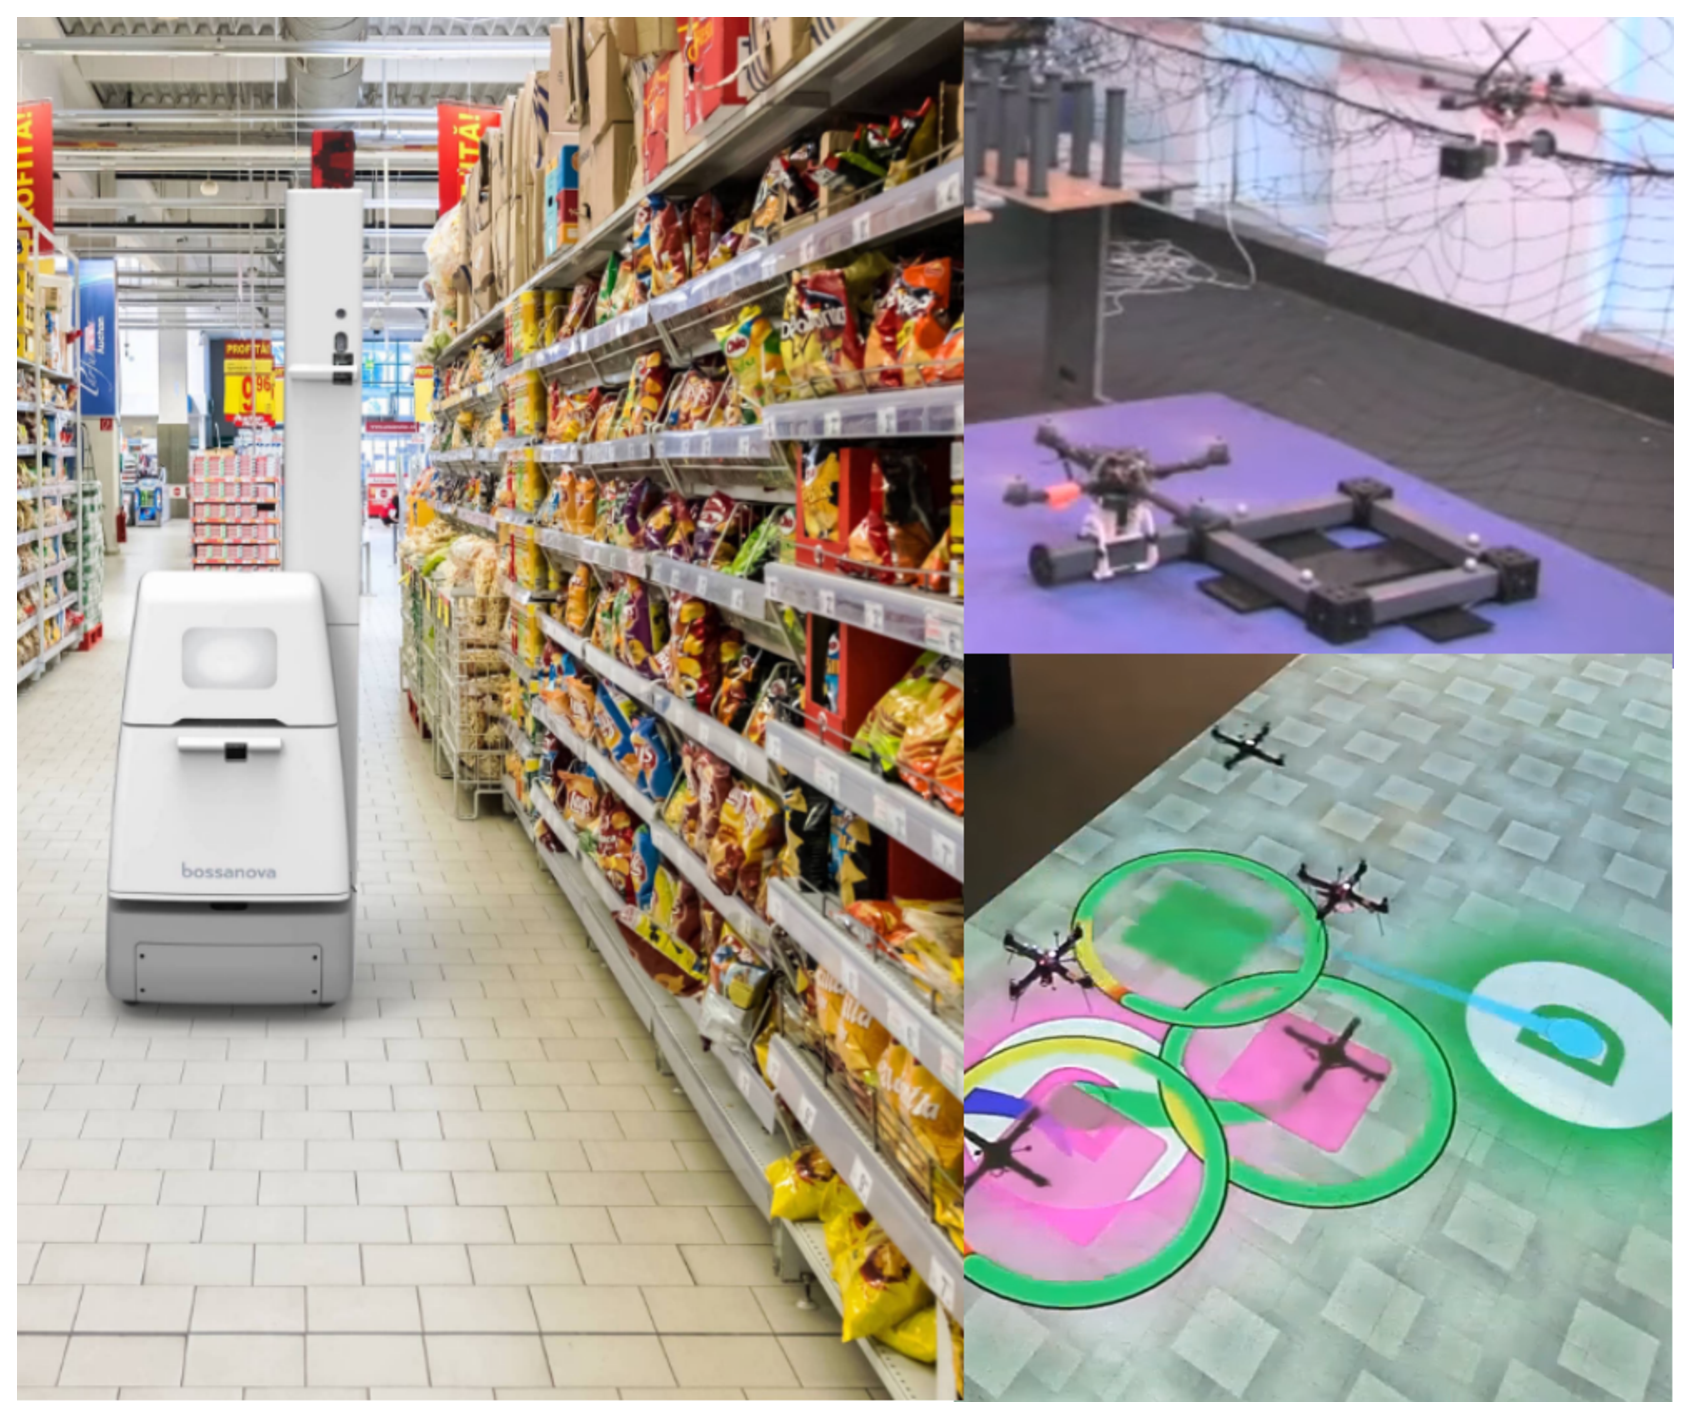
\includegraphics[width=\textwidth]{Chapters/figures1/swarm_safe.eps}
\label{fig:intro}
\caption{Clockwise from left: 1) A mobile robot navigating in a retail store to provide inventory solutions. They are designed to collaborate with other robots at the end of scanning an aisle. 2) Swarm of robots teaming up in a cooperative task of building lego blocks at Grasp Laboratory, University of Pennsylvania. 3) Decentralized control and planning of a multi-robot system at University of New Hampshire.}
\end{figure}

\section{Thesis}

My thesis in this dissertation is the following:

\begin{center}
\textit{Ordering the variables of the fused factor graph using the ordering of the parent factor graphs provides a superior alternative to the complete reordering approach that is fast, efficient and also numerically stable. Also, by introducing the concept of ``global nail" the issue of relative pose graph initialization for different robots is solved.}
\end{center}

\paragraph{}
I split this thesis into three claims that correspond to the Chapters \ref{chap:three}, \ref{chap:four} and  \ref{chap:five} respectively. The goal of my research is efficient factor graph fusion, globally consistent pose initialization for all the robots and rapid multi-channel object detection as explained below:

\begin{enumerate}
\item \textit{Fused Graph Ordering:} Variable reordering is a technique used to retain the sparsity of the factor graph during its factorization. This chapter proposes a numerically stable variable ordering strategy for the fused graph by reusing the parent graph ordering that is faster than the naive approach of complete reordering (Chapter \ref{chap:three}). 

\item \textit{Multi-robot Pose Graph Initialization:} Factor Graph is also referred as Pose Graph in the SLAM context. This chapter introduces a new type of error function used as a factor in the factor graph to estimate the globally consistent trajectory for the robots starting at unknown relative initial positions.

\item \textit{Multi-robot Data Association:} This is another common problem in multi-robot mapping that deals with unknown robot identity during a robot-robot encounter. The experimental real world dataset has colored fiducials attached to the robots and the environment. An improved version of Viola-Jones rapid detection \cite{violajones} for identifying the fiducials is developed and the computational complexity is studied (Chapter \ref{chap:five}). 
\end{enumerate}

\paragraph{}
In the reminder of this chapter, I lay down the reasoning leading to my thesis.

\section{Efficient Factor Graph Fusion}
In order to be useful for a multi-robot system, SLAM needs to perform at real-time. Offline or batch solutions to SLAM means the robot has to wait until the calculation for the update is finished. Even in the case of multiple robots with a centralized mapping capability, quicker update times are always useful. With the centralized system calculating the best estimate based on measurements received from all the robots, an update sent back to the individual robots could be used to correct or improve the local estimates. 

\paragraph{}
A real-time algorithm should also be able to update the system incrementally. This means that the centralized system should just require the new set of measurements from the individual robots taken after the last time they communicated to make an update. SLAM by nature itself is a sparse problem with the measurements connected temporally almost always. The centralized system should also be able to calculate an update by just using a local portion of the graph being impacted by the new measurements. For example, the measurements from a robot moving down a particular aisle in a retail store are completely independent of the measurements and observations made in a different and far away aisle. So a centralized system recalculating the estimates of the unaffected portions of the map is not a wise option. This incremental requirement for SLAM problem is well studied, particularly by Kaess and Dellart in \cite{kaessisam} and \cite{kaessisam2}. By using the formulation presented in their work and reusing the variable ordering of the graph being combined we come up with an efficient graph fusion strategy (Chapter 3). 

\section{Multi-robot Pose Graph Initialization}
The measurements from multiple robots must be globally consistent to build a unified map of the environment. In order to do this, all the robots should have a prior knowledge about their relative initial positions. It is not necessary or a fair assumption to consider that all the robots of a multi-robot system start at the same position on the map. Any arbitrary value to the initial position will lead to a conflict during a robot-robot encounter in terms of global map alignment. For example, in the case of multiple robots navigating in a large retail store across distinct aisles, lack of knowledge about each robot's initial position gives the freedom to all the independent trajectories to align together in several possible ways. Although there is a closed form solution to resolve the alignment issue with a single robot-robot encounter \cite{zhoumulti} the devised algorithm should be able to continuously and incrementally integrate the incoming measurements to refine the alignment error. 

\paragraph{}
The encounter could also be \textit{indirect} in which multiple robots visit the same portion of the environment at different time instants. In this case, the variable representing the pose of the landmark (or common portion of visit among different robots) is also involved in alignment estimation. It is therefore essential for the algorithm to incorporate indirect encounters in the alignment of the map. In other words, aligning the map is same as finding the globally consistent initial pose for all the robots. A cost function that tries to minimize the alignment error and also supports multiple encounters between the robots is formulated and optimized in Chapter 4.

\section{Multi-robot Data Association}
Data Association, in general, is an important component of SLAM. It is the process of recognizing previously visited landmarks in the environment to refine the map and the robot's path. There are several ways of extracting the features of interest (landmarks) from the environment, ranging from wireless network-based to computer vision techniques. With multiple robots in place the identity of the fellow robots should also be identified on top of the landmarks in the environment. The data association engine should be able to recognize both the landmarks in the environment and the robot IDs from the extracted features. Simultaneously, these type of sophisticated measurements should not consume a large amount of time as it introduces the problem of synchronization and scheduling.

\paragraph{}
In this thesis, an object detection based data association is used to demonstrate the results with the experimental dataset. Although this is not the main concentration of the thesis, an improved Viola-Jones rapid object detection \cite{violajones} is devised to work in the multi-channel image space. As it is able to use multiple image channels beyond color (like depth and intensity), detection could be performed at a much lower resolution saving time per scan. Chapter \ref{chap:five} presents a theoretical study of the time complexity of the improved algorithm.

\section{Organization}
The remainder of the dissertation is organized as follows: The background and related work is discussed separately for factor graph ordering and multi-robot map alignment in Chapter 3 and Chapter 4 respectively. The next chapter formally introduces the factor graph and the Bayes tree data structure often used throughout my work. In Chapter \ref{chap:two}, a set of key terminologies from graph theory and sparse linear algebra literature are also explained for the sake of better understanding and completeness. The novel algorithm to quickly find the variable ordering of the fused graph is presented in Chapter 3. Experimental results on the standard real world datasets from the sparse linear algebra literature is also presented at the end of Chapter 3. Chapter 4 deals with the problem of pose graph initialization or map alignment and gives a solution by devising an appropriate cost function and ``global nail". A detailed numerical section, sensor models $\&$ software library used and demonstration of experiments is presented in Chapter 5. The conclusions and the potential future work are also discussed in the same chapter. Finally, Chapter \ref{chap:five} presents the improved rapid object detection for multi-channel images.





 % Introduction

\chapter{Factor Graphs and Bayes Tree}

In this chapter, I will introduce several key basic concepts and the associated terminologies of \textit{factor graph} \cite{factorgraph} along with its SLAM formulation as proposed by Kaess and Dellart [ref] but for the scenario of multiple robots. A factor graph is a type of probabilistic graphical model which represents the factorization of a probabilistic distribution function. They are used to model complex estimation problems having wide range of applications in robotics. Formulating the SLAM problem using the factor graph, also known as pose graph in the robotics literature, opens the door for the application of several probabilistic inference algorithms. Our research is multi-robot SLAM and we will use this as an example throughout the paper. In the case of SLAM, the set of constraints obtained from the proprioceptive sensors like odometry measurements, inertial measurement units (IMUs) and exteroceptive sensors like range (LIDAR) and vision measurements form a Markov chain that connects all the variables to be estimated. Also, the solution to the SLAM problem using the recent pose graph representations has garnered much attention because of their computational efficiency and robustness. 





 % Background Theory 

\chapter{Efficient Factor Graph Fusion}
\label{chap:three}

%In order to be useful for the mobile robots, SLAM needs to perform at real-time. Solving the SLAM problem represented by a factor graph proceeds by optimizing the equivalent nonlinear least-squares problem \cite{lumiliosfirstgraphslam}. The sparsity of the underlying graph structure makes the optimization tractable at real-time. During factorization the sparsity of the graph is retained using a technique widely known in the sparse linear algebra and graph theory community called variable reordering. Variable ordering or Elimination ordering is the order in which the variables are eliminated while solving a system of linear equations. A good ordering is necessary to avoid fill-in which refers to the additional non zero entries produced out of factorization. In case of a multi-robot scenario, factor graphs of the individual robots are fused/combined to improve the overall estimate. This requires finding the variable ordering of the fused factor graph. 
%Chapter 3 comes up with a methodology to quickly find the variable ordering of the combined graph using the ordering of the participating factor graphs. The worst case here would be to do a complete reordering of the fused graph. We provide a complexity analysis to compare the time performance of both the options. Also, fusing and factorizing the graph during multi-robot SLAM optimization for best estimate requires coming up with a variable ordering for the fused graph. Factorizing/Solving a factor graph proceeds by generating a order of elimination for the variables called variable ordering or elimination ordering. In case of a multi-robot scenario while combining the factor graphs to improve the overall estimate the variable ordering of the participating factor graphs can be used to quickly find the variable ordering of the resultant combined factor graph. To do this, we use the Bayes Tree \cite{kaessbayestree} representation of the factor graph which also gives access to the subset of variable that gets affected on combining the parent factor graphs. 
In the previous chapter, I described how the multi-robot smoothing and mapping is formulated as a least squares problem with a flavor that is specific to our implementation. Following that, I discussed the options to incrementally solve the least squares optimization and the critical requirement for fast, efficient and incremental variable reordering. A good ordering is necessary to reduce the amount of fill-in which refers additional non-zeros introduced during elimination. However, it has been shown that finding an optimal ordering for an arbitrary factor graph is NP-complete \cite{orderingnphard}. An optimal ordering called perfect elimination ordering \cite{chordaloptimalordering} exists only if the factor graph is chordal. SLAM graphs are generally \textit{not} chordal mainly due to revisiting the landmarks after a long time and loop closures that connect two far away nodes. Loops in the trajectory can result in a significant increase in computational complexity through a large increase of non-zero entries in the factor matrix. In addition to the typical loop closures in the SLAM problem, a multi-robot scenario could introduce several non-trivial loop closures. This is because for an indirect encounter between the robots, a big chunk of graph with several measurements from one robot has to combined with a far away node of another robot. Such an update is equivalent to loop closure in terms of computation and storage. Despite that, it is important in a multi-robot scenario to fuse the factor graphs of individual robots to improve the overall estimate. This requires finding the variable ordering of the fused factor graph.
\paragraph{}
To combat this scenario, this chapter comes up with a methodology to quickly find the variable ordering of the combined graph using the ordering of the participating factor graphs. The worst case here would be to do a complete reordering of the fused graph. We provide a complexity analysis to compare the time performance of both the options. The outline of this chapter is as follows: In the next section, I will provide a relevant literature survey from linear algebra and graph theory community. Following that, I will dive deep in to Bayes tree data structure that was introduced in the previous chapter to establish incremental variable ordering. Then I will formally verify that the proposed ordering does not violate any of the standard rules to be obeyed. Finally, I will explain the proposed approach and display results on a standard dataset from sparse linear algebra community.

\section{Related Work} 
Solving the least-squares and linear programming problem is central to several scientific  and engineering applications. Our focus in on sparse least-squares optimization with primary applications to SLAM. Smoothing formulation of SLAM as a least-squares with sparse graphs was first done by Lu and Milios \cite{lumiliosfirstgraphslam}. Their method provides both batch and sequential procedure but performs the expensive inversion of the information matrix for updates. Although several smoothing based SLAM solutions have been developed based on conjugate gradient \cite{cgdescent}, gradient descent \cite{gdescent}, relaxation \cite{thrunprobabilistic} and multi-level relaxation \cite{mlrelaxation}, we only deal with the ones that derive performance improvements from information matrix decomposition. $\sqrt{SAM}$ by Dellaert \cite{dellaertonlysam} was the first work to replace expensive matrix inversion with sparse matrix factorization for the SLAM problem. It mentioned the dramatic performance improvements that could be derived from good variable ordering but is done only on a batch setting. The two key algorithms that improved on the least-squares formulation of SLAM using the premise set by \cite{dellaertonlysam} include ISAM \cite{kaessisam} and ISAM2 \cite{kaessisam2}. Both of these works combine the formulation in \cite{lumiliosfirstgraphslam} with the interchangeable linear algebra and graph theory flavor introduced in \cite{dellaertonlysam} and provide some additional improvements in terms of incremental optimization. Recently, Agarwal and Olson \cite{variableorderingslam} provided different variable reordering strategies to SLAM and explained the critical role played by variable ordering in different solutions to SLAM. 
\paragraph{}
In our work, we use ISAM2 using the Bayes tree \cite{kaessbayestree} \cite{kaessisam2} as the underlying state estimation engine because it is exact, incremental and solves the full non-linear problem. While tremendous amount of work is done to extend the general SLAM algorithms to multiple robots, smoothing and mapping for multi-robot SLAM is not explored much. The most relevant ones include \cite{multipleisam} by Kim \textit{et al.}, C-SAM \cite{csam} and Tectonic SAM \cite{tectonicsam}. Although these algorithms are based on Smoothing and Mapping, Tectonic SAM addresses only single robot, batch mapping and the other two algorithms only address the fundamental multi-robot mapping issues like map-aligning and relative pose initialization. Important graph based SLAM approaches that build independent sub-graphs and merge those graphs include \cite{gdescent}, \cite{fresetreemap} and \cite{freseclosing}.  Folkesson's \cite{gdescent} reduces the graph complexity by collapsing parts of the robot trajectory into a cluster called star-nodes. Frese's \cite{fresetreemap} and \cite{freseclosing} gives a hierarchical approach by exploiting the square root information and representing the Cholesky factors as a tree data structure. They provide a highly efficient algorithm but employ numerous approximations and none of these partition based algorithms are extended to multi-robots. Also, several recent developments in the algebraic graph theory community like hypergraph nested dissection ordering \cite{hund} and exact graph partitioning algorithm \cite{exactordering} have not been utilized in solutions for SLAM. Clearly from the above discussion, previous research has either been done in graph merging for single robot SLAM or, multi-robot SLAM that does not deal with combining the graphs. 
\paragraph{}
While solving large linear systems, it is a very common preprocessing step to order the columns of the matrix $A$ to be factorized to keep the factorization as sparse as possible. Finding the variable ordering involves finding the permutation matrix $P$ which is right-multiplied with $A$ to obtain the ordered matrix $AP$. Cholesky or QR factorization of $AP$ is more sparser and requires less storage than factorizing $A$. Ordering schemes have been proposed for different class of problems that include - 1) $A$ being symmetric 2) $A$ being unsymmetric. As finding the optimal ordering is NP-complete \cite{orderingnphard} various heuristics have been developed. The common aspect across all the approaches is to eliminate the nodes in the ascending order of their degrees. This is called as the minimum degree algorithm which is derived from a method first proposed by Markowitz in 1957 \cite{markowitzelimination} for non-symmetric linear programming problems. The symmetric matrix version was formalized by Tinney \textit{et al.} \cite{tinneyfirstordering}. The ordering of the nodes directly on the graph data structure was derived by Rose \cite{rosegraph}. Initial algorithms for symmetric matrices also include approximate minimum degree (AMD) \cite{amd} and nested dissection \cite{nesdis}. In case of the unsymmetric matrix such as Jacobian $A$, it is converted to symmetric information form $A^\top A$ to be used by these ordering schemes. State-of-the-art algorithms like column approximate minimum degree ordering (COLAMD) \cite{colamd} works directly on the non-zero pattern of $A$ without explicitly calculating $A^\top A$. A brief survey of the evolution of minimum degree ordering is consolidated by George \cite{georgeevolution}. Nested dissection is a divide and conquer heuristic based on graph partitioning that has the advantage of reordering the matrix into a form suitable for parallel execution. Very recently, nested dissection has been extended to unsymmetric hypergraphs in \cite{hund}. Although there is a significant amount of research in developing a near to optimal variable ordering tailored for various graphical models, to the best of our knowledge, there is no work in finding an ordering for the graph obtained by fusing ordered graphs. 

\section{Bayes Tree for Variable Ordering}
Topologically, the Bayes net described in Section \ref{sss:bayes_net_intro} is a chordal directed acyclic graph. By identifying cliques (groups of fully connected variables), the Bayes net may be rewritten as a Bayes tree. For full details about the clique-finding algorithm, see Kaess et al. \cite{kaessbayestree}. Within the Bayes tree, each node represents the conditional density of the clique variables (also called as frontal variables), $\Theta_j$, given all of its neighbors (also called as separators), $N(\Theta_j)$:
\begin{equation}
p(\Theta) = \Pi(\Theta \mid N(\Theta_j))
\end{equation}
During elimination of the factor graph (assuming the Bayes net is formed), the leaves of the tree are built first, and factors on the conditional variables are passed up the tree to their parents. Back-substitution then proceeds top-down from the root clique, which is eliminated last, as it has no external dependencies. The solution of the frontal variables of the parent clique are passed down the tree to the children, which are guaranteed to depend only on the frontal variables of their ancestors. 
\begin{figure}
\centering
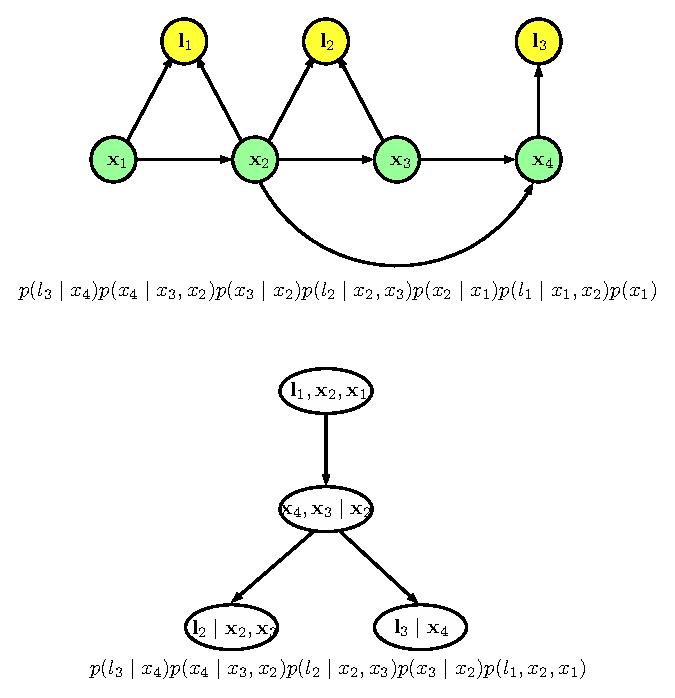
\includegraphics{Chapters/figures3/bn_bt_factorization_vert}
\caption{Bayes network and Bayes tree representations of the factor graph example used in last chapter with the elimination order $O = [l_3, l_2, l_1, x_4, x_3, x_2, x_1]$. The factorization of the factor graph joint probability density is mentioned for both the representations.}
\label{fig:bn_bt_factorization}
\end{figure}
\paragraph{}
Like the Bayes net, the structure of the Bayes tree is affected by the selected variable ordering. The Bayes net and Bayes tree representations are interchangeable. This is shown in the Figure \ref{fig:bn_bt_factorization} with the factor graph example used in Section \ref{ss:fg_to_bn_to_bt}. The terms $p(l_3\mid x_4)$, $p(x_4 \mid x_3, x_2)$, $p(x_3 \mid x_2)$, $p(l_2 \mid x_2, x_3)$ are present in both the factorizations. It can be shown using the chain rule in Bayes theorem that $p(l_1, x_2, x_1) = p(l_1 \mid x_1,x_2)p(x_2\mid x_1)p(x_1)$. Although both the representations are same given the variable ordering, modeling the inference using a tree structure is often more convenient and intuitive: elimination passes information up the tree, while back-substitution propagates information down the tree.
\paragraph{}
At every iteration, the update can be a new variable to be added to the graph or a new measurement factor connecting already existing variables. In both the cases, the square-root information of several variables other than the new variable in different cliques of the Bayes tree has to be updated. This could either be done by 1) Going back to the factor graph, adding a new measurement and/or a variable, reordering all the variables and completely factorizing the graph from scratch or 2) Partially recovering the portion of factor graph to which the new measurement and/or a variable should be added, reordering the partial graph and factorizing it. The second option is incremental, efficient and hence preferable, but would require the knowledge of subset of variables and factors that gets affected on touching a variable. This is exactly obtainable from the formulation of the Bayes tree.
\paragraph{}
A new variable is always accompanied by a measurement. When a new measurement is added, for example a factor $c^\prime(x_j,x_{j^\prime})$, only the paths between the cliques containing $x_j$ and $x_{j^\prime}$ (respectively) and the root are affected. The sub-trees below these cliques are unaffected, as are any other sub-trees not containing $x_j$ or $x_{j^\prime}$. The example in Figure \ref{fig:bt_add_var} demonstrates the addition of a new pose node to the factor graph and Bayes tree example used in the previous chapter in Figure \ref{fig:bn_to_bt}.
\begin{figure}
\centering
\includegraphics[width=\textwidth]{Chapters/figures3/bt_add_new_variable}
\caption{Adding a new variable with measurement to a factor graph example described in the previous chapter. It should be noted that only a part of the Bayes tree (red filled nodes) to which the new variable is added is recovered, reordered and factorized. The unaffected cliques (purple filled nodes) are attached back to the new tree. The new variable added is shown used a red broken circle.}
\label{fig:bt_add_var}
\end{figure}
\paragraph{}
This in turn may move the estimates far off the current linearization point or add new non-zero components to the square-root factor. The former would require updating the linearization point and the latter requires reordering the variables. But as the set of variables that will be affected is known in advance it could be leveraged by changing the linearization point or reordering and factorizing only those variables. This relationship is understood by the construction of Bayes tree and was not obvious within the matrix framework \cite{kaessbayestree}.  
\subsection{Multi-robot Pose Graph Fusion}
From the construction of the Bayes tree discussed so far and the example in Figure \ref{fig:bt_add_var} it is clear that the Bayes tree is suitable for updating the square-root information incrementally. With ISAM2 \cite{kaessisam2} as the SLAM algorithm, a centralized cooperative mapping system will require fusing the maps from individual robots represented as the Bayes tree. In case of centralized mapping it could be assumed that every robot's factor graph is accessible always with no restrictions on bandwidth or that the robots share information only when they encounter. For our experiment, we assume that the robots share information only when they encounter. Also, our procedure does not require both the robots to identify each other when they encounter and work even if one robot identifies the other. Knowing the subset of variables using the Bayes tree which alone can be reordered could easily be extended to the situation of fusing multiple robots' pose graphs. 
\paragraph{}
Direct encounters between robots introduce a constraint between the cliques of two different Bayes tree with pose nodes as the frontal variables. As a direct encounter relates the recent pose of the robots, the constraint joins the nodes near the root of the tree. The argument that the recent poses of the robot need not necessarily end up near the root of the tree after variable ordering will be addressed later. Since a connection is made between the nodes near the root of the tree the total number of affected variables is minimal. Whereas an indirect encounter occurs when two robots observe the same part of an environment (not necessarily at the same time), allowing a constraint of type robot-landmark-robot between the robot poses pivoted by the landmark pose, to be estimated. They could also be transformed into a constraint between the positions of two robots at the respective time steps. This type of constraint connects the recent pose of one of the robots from which the landmark is observed with a older pose of another robot from which the same landmark was observed. Figure \ref{fig:fusing_bt} gives a pictorial step-by-step procedure to combine two Bayes trees.
\begin{figure}
\centering
\includegraphics[height=\textheight,width=\textwidth]{Chapters/figures3/fusing_bt}
\caption{Fusing multiple Bayes trees to calculate the best estimate. Only the affected part (inside blob in row 3) of both the Bayes trees are recovered and refactorized. $O_1$, $O_2$ and $O_{fused}$ are the variable ordering of first, second and the fused factor graph.}
\label{fig:fusing_bt}
\end{figure}
\paragraph{}
In Figure \ref{fig:fusing_bt}, the factor graph of two robots exploring the environment is considered. Row 3 indicates the equivalent Bayes tree based on some variable ordering $O_1$ and $O_2$. It can be seen from the common variable among the factor graphs that both the robots have visited the same landmark $l_1$. To fuse those Bayes trees, only the path between the clique containing the landmark frontal variable and root clique is recovered as factor graph. The factor graph centred over the common variable is fused, reordered and eliminated back into a Bayes tree. The unaffected portions of the individual Bayes tree is merged back. These unaffected portions are shown as colored cliques in row 3 of Figure \ref{fig:fusing_bt}. While merging back the unaffected portions, the clique containing the earliest eliminated variable out of all the conditional variables of the unaffected clique is considered as the parent clique. For example, in Figure \ref{fig:fusing_bt}, it can be seen in the second Bayes tree that the unaffected green colored clique with frontal variable $\textbf{x}_1^2$ has two conditional variables $\textbf{x}_2^2$ and $\textbf{x}_4^2$. It is attached to the clique containing the earliest eliminated variable, according to $O_2$, as the frontal variable, $\textbf{x}_2^2$. However, in row 5 containing the fused Bayes tree, the same unaffected clique is attached to the clique with frontal variable $\textbf{x}_4^2$ as it is eliminated before $\textbf{x}_2^2$ according to $O_{fused}$. The idea here is that, during elimination information is propagated up the tree and every eliminated variable will have the variables yet to be eliminated as its ancestor if there is a fill-in between them.

\section{Formal Verification}
Before proceeding to the proposed algorithm, it is important to formally validate that the operations carried out and the utilization of Bayes tree does not violate any of the standard assumptions, works for any general class of factor graph problems and is backward compatible. Firstly, when multiple robots visit several same regions of the environment the number of common landmarks between the graphs go up. The Bayes tree would be used to extract the affected subset of variables when combining the graphs with multiple common variables. It has to be verified that these affected subset of variables do not form disconnected components. Secondly, it has to be ensured that the root clique always contains more than one frontal variable. This is needed both in terms of the property of the Bayes tree and the requirements of the software optimizer used by us, \cite{gtsamhandson}. To ensure these the following two proofs are given:
In the following write-up a variable in/of the clique usually refers to the frontal variable of the clique. Let us consider the simple case of merging two bipartite graphs $\mathcal{G}_1 = (\mathcal{C}_1, \Theta_1, \mathcal{E}_1)$ and $\mathcal{G}_2 = (\mathcal{C}_2, \Theta_2, \mathcal{E}_2)$ with their Bayes tree function given as $\mathcal{B}_i(\mathcal{C}_{i})$. The Bayes tree function returns the union of set of variables in the ancestor cliques of the clique containing each and every variable in $\mathcal{C}_{i}$, $i = 1,2$ here. The graph is merged only when the set of common variables $\mathcal{C}_1 \cap \mathcal{C}_2 \neq \emptyset$. The set of all affected variables obtained from the Bayes tree is given as $\mathcal{C}^{fused} = \mathcal{B}_1(\mathcal{C}_{1}) \cup \mathcal{B}_2(\mathcal{C}_{2}) \cup (\mathcal{C}_1 \cap \mathcal{C}_2)$. The fused graph is then given as $\mathcal{G}^{fused} = (\mathcal{C}^{fused}, \Theta^{fused} ,\mathcal{E}^{fused})$ where $\mathcal{E}^{fused} = \{ (u,w) \mid [u,w \in \mathcal{C}_1 \cap (u,w) \in \mathcal{E}_1] \cup [u,w \in \mathcal{C}_2 \cap (u,w) \in \mathcal{E}_2] \}$ and $\Theta^{fused} = \{ \theta(u,w) \mid \theta \in \Theta_1 \cup \Theta_2; u, w \in \mathcal{C}_1 \cup \mathcal{C}_2 \}$.
\begin{theorem}
The set of affected variables from the Bayes tree do not form a disconnected graph.
\end{theorem}
%\paragraph{Proof 1:} \textit{The set of affected variables from the Bayes tree do not form a disconnected graph.}\\
\begin{proof}
The common variables forming the separator when combining the factor graphs can have multiple connected components. However, the  subset of affected variables obtained by recursively traversing up the Bayes tree from every common variable forms a single connected component. It follows from the fact that, although the common variables might be present at different leaf cliques or non-leaf cliques, different branches or different depths, they all have a single root clique. Recovering all the common variables with all its ancestors will eventually be connected by the frontal variables of the root clique. It is mathematically verified by showing that the multiplicity of 0 as an eigenvalue of the Laplacian matrix of the fused graph is 1. The Laplacian matrix $\mathcal{L}_{{N\times N}}$ of a bipartite factor graph with $N$ variable nodes is given as:
\begin{equation}
\mathcal{L}^{fused} = \mathcal{D}^{fused} - \mathcal{A}^{fused}
\end{equation}
where $\mathcal{D}$ is the degree matrix and $\mathcal{A}$ is the adjacency matrix of the graph. Simplifying the above equation:
\begin{equation}
{\displaystyle \mathcal{L}_{j,k}:={\begin{cases}\deg(v_{j})&{\mbox{if}}\ j=k\\-1&{\mbox{if}}\ j\neq k\ {\mbox{and}}\ v_{j}{\mbox{ is adjacent to }}v_{k}\\0&{\mbox{otherwise}}\end{cases}}} 
\end{equation} 
So from the above general equation it can be seen that $\mathcal{L}^{fused}$ is a square matrix of size $\mid \mathcal{C}^{fused} \mid$ with the degree, $deg(\mathcal{C}_n)$; $n = 1 \ldots N$, along its diagonals. The degree of a variable node is equal to number of edges that are incident to it from other variable nodes. This is also equal to the number of negative ones in every column other than the diagonal element as the number of adjacent variable nodes is equal to degree of the node. Therefore a row transformation such as $R_1 = R_1 + R_2 + \ldots + R_n$ will result in all-zeros in row 1. Hence, the Laplacian matrix is rank deficient and the determinant is zero. It follows from the Invertible Matrix Theorem (IMT) \cite{imt} that a $\mathcal{L}_{{N\times N}}$ matrix is invertible if and only if 0 is not an eigenvalue of $\mathcal{L}_{{N\times N}}$. But as the rank goes down by 1 (not more than one row could be zeroed by this transformation), only the constant term vanishes from the characteristic polynomial while finding the eigenvalues. Hence the multiplicity of 0 in the eigenvalue multiset is 1 which equals the number of connected components. This proves that the set of affected variables forms a connected graph. In other words, the set of affected variables from the Bayes tree do not form a disconnected graph.
\end{proof}
\begin{theorem}
On fusing the graphs, the root clique of the Bayes tree will have more than one frontal variable.
\end{theorem}
\textit{\textbf{Lemma:}} There is always a path between two nodes in the fused factor graph.
\begin{proof}
It naturally follows from the previous theorem that the fused factor graph forms a single connected component and the well known fact that any two nodes are joined by a path in an undirected graph.
\end{proof}
\textit{\textbf{Lemma:}} The edge between the last and last but one node always fills-in, if all the nodes between these two nodes are eliminated before these two nodes.
\begin{proof}
The concern here is that variable ordering an arbitrarily mixed graph should not defy the standard norms of the root clique. Let the factor graph obtained by joining that of two robots be the one obtained from a single robot exploration task itself. Structurally, the fused factor graph is not any special when compared to the individual graphs. So any variable ordering is valid but may end up with a high fill-in. In the equivalent matrix representation, every column eliminated will leave changes with the rest of the columns yet to eliminated. By proceeding this, the last but one column in the elimination order will leave the information (make changes) with the last column to be eliminated. This information left by the last variable to the last but one variable is represented by an arrow pointing to from the last variable node to the last but one variable node. Therefore there is always a factor of the form $p(last \ but \ one \ variable \mid last \ variable)$ at the second iteration of clique-finding algorithm which forms the root clique with these nodes as the frontal variables. 
\end{proof}

\section{Ordering the Fused Graph}
\label{sec:fusion_ordering}
Let $\mathcal{G}_1 = (\mathcal{C}_1, \Theta_1, \mathcal{E}_1)$ and $\mathcal{G}_2 = (\mathcal{C}_2, \Theta_2, \mathcal{E}_2)$ be two bipartite factor graphs that has to be fused. The Bayes tree function $\mathcal{B}_i(\mathcal{C}_{i})$ is same as that defined in the previous section. Let $O_1$ and $O_2$ be the COLAMD \citep{colamd} orderings of $\mathcal{G}_1$ and $\mathcal{G}_2$ respectively. The factor graphs $\mathcal{G}_1$ and $\mathcal{G}_2$ are eliminated based on the ordering $O_1$ and $O_2$ as explained in Section \ref{ss:fg_to_bn_to_bt} and stored as the Bayes tree \cite{kaessbayestree}. Let $\mathcal{C}_{common} = \mathcal{C}_1 \cap \mathcal{C}_2$ represent the set of common variables among the graphs. We inherit the definition of $\mathcal{C}^{fused}$, $\Theta^{fused}$ and $\mathcal{E}^{fused}$ from the previous section that gives the fused graph $\mathcal{G}^{fused} = (\mathcal{C}^{fused}, \Theta^{fused} ,\mathcal{E}^{fused})$. The set of variables that get impacted are obtained from the Bayes tree as $\mathcal{C}^{affected}_1 = \mathcal{B}_1(\mathcal{C}_{common})$ and $\mathcal{C}^{affected}_2 = \mathcal{B}_2(\mathcal{C}_{common})$. It should be noted that $\mathcal{C}^{affected}_1 \cap \mathcal{C}_{common} = \emptyset$, $\mathcal{C}^{affected}_2 \cap \mathcal{C}_{common} = \emptyset$ and $\mathcal{C}^{fused} = \mathcal{C}^{affected}_1 \cup \mathcal{C}^{affected}_2 \cup \mathcal{C}_{common}$. 

\subsection{Fusion Ordering}
Ordering a fused graph is same as finding the permutation matrix $P_1$ that has to be post-multiplied with the factor graph matrix or the Jacobian matrix $A$. A permutation matrix is a square binary matrix that has exactly one entry of 1 in each row and each column and 0s elsewhere. The graphs of multiple robots are fused only when there are common variables among them, $\mathcal{C}_1 \cap \mathcal{C}_2 \neq \emptyset$. Let the ordering $O_1 = [o^{c^1_1}_1, o^{c^2_1}_1, \ldots, o^{c^{n_1}_1}_1]$ and $O_2 = [o^{c^1_2}_2, o^{c^2_2}_2, \ldots, o^{c^{n_2}_2}_2]$ where $n_1=\mid \mathcal{C}_1 \mid$, $n_2=\mid \mathcal{C}_2 \mid$, $\{ c^1_1, c^2_1, \ldots , c^{n_1}_1 \} \in \mathcal{C}_1$ and $\{ c^1_2, c^2_2, \ldots , c^{n_2}_2 \} \in \mathcal{C}_2$. Consider the functions $o_1(v)$ and $o_2(v)$ that gives the ordering value of the variable $v \in \mathcal{C}_1$ and $v \in \mathcal{C}_2$ respectively. For instance, $o_1(c_1^{n_1}) = o^{c^{n_1}_1}_1$. With these notations, the relative ordering of the fused graph, $\mathcal{G}_{fused}$ is derived below. 
\paragraph{}
The relative ordering of the $\mathcal{C}_1^{affected}$ variables of the $\mathcal{G}^{fused}$  graph is given as:
\begin{equation}
O^{fused}_1 = arg \ \text{sort}\biggl( \bigcup_{j \in \mathcal{C}_1} o_1(j) \biggr)
\end{equation}
where \textit{arg}sort gives the original position of each element in the sorted array. For example, the above operation on the array $[41, 23, 12, 8, 22]$ gives $[4, 3, 5, 2, 1]$. The relative ordering of the $\mathcal{C}_2^{affected}$ variables of the $G^{fused}$  graph is given as:
\begin{equation}
O^{fused}_2 = \mid O_1^{fused} \mid + arg \ \text{sort}\biggl( \bigcup_{j \in \mathcal{C}_2} o_2(j) \biggr)
\end{equation}
The common variables are positioned towards the end of the ordering and are eliminated at last:
\begin{equation}
O^{fused}_{common} = \mid O_1^{fused} \mid + \mid O_2^{fused} \mid + arg \ \text{sort}\biggl( \bigcup_{j \in \mathcal{C}_{common}} o_{common}(j) \biggr)
\label{eq:fused_ordering}
\end{equation}
Thus, using the parent orderings of the graphs $\mathcal{G}_1$ and $\mathcal{G}_2$ the relative ordering of $G^{fused}$ is given by the concatenated array $O^{fused}  = [ O_1^{fused}, O_2^{fused}, O_{common}^{fused}]$. The permutation matrix $P^1 \in [0,1]^{\mid N \mid \times \mid N \mid}$ and $\mid O^{fused} \mid = N$ where $N = \mid O_1^{fused} \mid + \mid O_2^{fused} \mid + \\ \mid O_{common}^{fused} \mid$. 
\begin{equation}
{\displaystyle P_{j,k}^1:={\begin{cases}1 &{\mbox{if}}\ j=O^{fused}_k \\0&{\mbox{otherwise}}\end{cases}}} 
\label{eq:permutation_matrix}
\end{equation}
Therefore, in an event of fusing the graphs containing common set of nodes, the variables can be ordered by finding the permutation matrix and post-multiplying with the factor graph Jacobian matrix. The fusion ordered factor graph is then factorized using QR decomposition to obtain the estimate on combining the information from multiple robots. This fused graph is then converted to the Bayes tree using the proposed ordering and attached back to the unaffected portion of the Bayes tree. In this way, the incremental updates could be generated by reusing the parent ordering.
\subsection{Relation with Nested Dissection}
The idea of reusing the variable ordering by finding the relative ordering was inspired from the working principle of nested dissection \cite{nesdis}. Although the principle of nested dissection has not been employed for reusing the variable ordering, in the SLAM context, it has been used for recursively partitioning the graph into multi-level submaps in \cite{nesdisslam}. Nested dissection is a fill-reducing ordering method based on the divide-and-conquer principle. It is a recursive algorithm that finds a graph separator at every iteration, which on removal splits the graph into multiple connected components. This process continues until a point at which the size of the connected components are small and ordering them is trivial. These simpler graphs in the leaf nodes  are ordered using some standard variable ordering technique like COLAMD \citep{colamd}. The backtracking starts by ordering the leaf nodes containing these smaller graphs first and continues till it reaches root node. By this process the nodes in the first separator are placed towards the end of the variable ordering. 
\paragraph{}
Reusing the variable ordering is similar to depth 1 nested dissection. Evidently, the nodes in $\mathcal{C}_{common}$ forms a separator that divides the graph $\mathcal{G}_{fused}$ into child graphs $\mathcal{G}_1^{affected}$ and $\mathcal{G}_2^{affected}$ where $\mathcal{G}^{affected}_i = (\mathcal{C}^{affected}_i, \Theta^{affected}_i ,\mathcal{E}^{affected}_i)$, $\Theta^{affected}_i \mid \{ \theta(u,w) = \theta \in \Theta_i; u, w \in \mathcal{C}_i \} $, $\mathcal{E}^{affected}_i = \{ (u,w) \mid u, w \in \mathcal{C}_i \cap (u,w)\in \mathcal{E}_i \}$. If the ordering of the graphs $\mathcal{G}_1^{affected}$ and $\mathcal{G}_2^{affected}$ could be reliably estimated using the parent ordering, the divide and conquer loop could be stopped and backtracked from depth 1 itself. This is exactly what is achieved by coming up with an ordering as per Equation \ref{eq:fused_ordering} and post-multiplying the Jacobian with the permutation matrix $P^1$ as given in Equation \ref{eq:permutation_matrix}.

\subsection{Numerical Stabilization}
Before explaining the approach that has been used to ensure numerical stability for matrix operations a few terminologies are introduced:
\paragraph{} 
\textit{Pivoting} is a common practise in matrix algorithms to add numerical stability to the final result. In the case of matrix algorithms, a pivot entry is usually required to be at least distinct from zero, and often distant from it; in this case finding this element is called \textit{pivoting}. Pivoting may be followed by an interchange of rows or columns to bring the pivot to a fixed position and allow the algorithm to proceed successfully, and possibly to reduce round-off error. Usually the element which has the largest absolute value in the pivot row or column is chosen as the pivot element. This is because the percentage error that accrues on using a $d$-digit arithmetic precision is as much lower as the absolute value is higher. Thus pivoting on the largest element propagates the smallest round-off errors possible.
\paragraph{}
Given a factor graph $\mathcal{G} = (\mathcal{C}, \Theta, \mathcal{E})$, a subset $\mathcal{M} \subseteq \mathcal{E}$ is defined as matching or assignment if no two edges of $\mathcal{M}$ are incident to the same node. In other words, it is a set of pairwise non-adjacent edges, \textit{i.e.} no two edges share a common vertex.
\paragraph{}
The proposed ordering described in the previous section only takes the structure into account, and not the numerical values. To stabilize the factorization and minimize pivoting, we wish to permute large entries to the diagonal. A standard approach is to model this as matching in the bipartite graph \cite{matching}. We use the matching permutation $P^2$ to permute the rows such that the large entries in every column resides on the diagonal. The remaining rows in the originally rectangular blocks have been “pushed down”. All the permutations applied on the matrix after this step should be symmetric. This permutation step for obtaining a strong diagonal is helpful for dynamic (partial) pivoting methods, since the number of row swaps is significantly reduced, thereby speeding up the factorization process \cite{matching}. It is essential for static pivoting methods, because it decreases the probability of encountering small pivots during the factorization.
\paragraph{}
In summary, the proposed fusion ordering and the numerical stabilization is applied on the fused graph or the fused Jacobian by post-multiplying and pre-multiplying the fusion ordering permutation matrix $P_1$ and the matching permutation matrix $P_2$.

\section{Experimental Results}
In this section, we present the experimental results of the proposed ordering algorithm when applied to the real world matrices. The algorithm was tested on a 2.3 GHz core i5 processor with 15.1 Gigabytes of memory. Figure \ref{fig:ordering_comparison_1} and \ref{fig:ordering_comparison_2} shows the non-zero structure of the square root factor for a bunch of real-world matrix datasets which are split and fused again using the standard COLAMD ordering \cite{colamd}, the relative fusion ordering (Section \ref{sec:fusion_ordering}) and the default order in which nodes of the graph are retrieved from the memory respectively. It can be seen from the $R$ matrix plot that the number of non-zeros are close to COLAMD ordering in the proposed ordering. At the same time, the gap in the number of non-zeros between the proposed ordering and the variable memory order is huge. It can be calculated that from these examples that, on an average the ratio of the difference between number of non-zeros in the proposed ordering and the variable memory order to the difference between the number of non-zeros in the proposed ordering and COLAMD ordering is 8.373. Also, it can be observed that just eliminating the variables in the order they are retrieved from the memory produces complete fill-in in some cases. 
\begin{figure}[!]
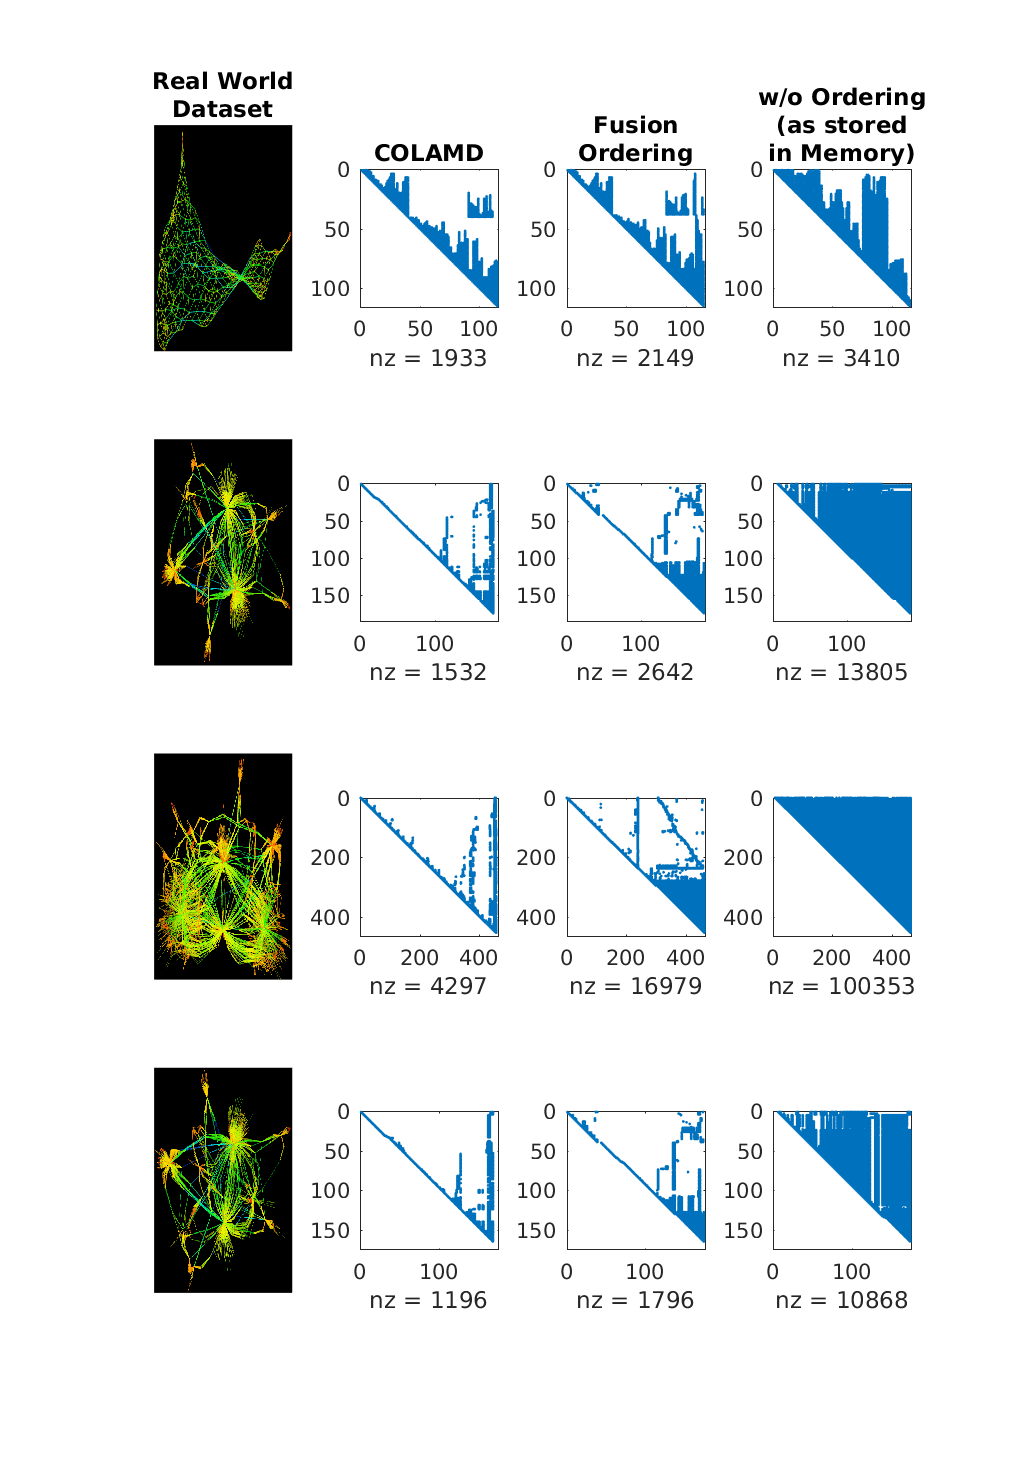
\includegraphics[width=\textwidth]{Chapters/figures3/ordering_comparison_1}
\caption{Comparison of number of non-zeros in the square root factor from QR factorization between the COLAMD ordering (second column), proposed ordering (third column) and the order in which the variables are retrieved (third column). The first column is the graph representation of the matrices in their lowest energy state \cite{suitesparse}.}
\label{fig:ordering_comparison_1}
\end{figure}
\begin{figure}[!]
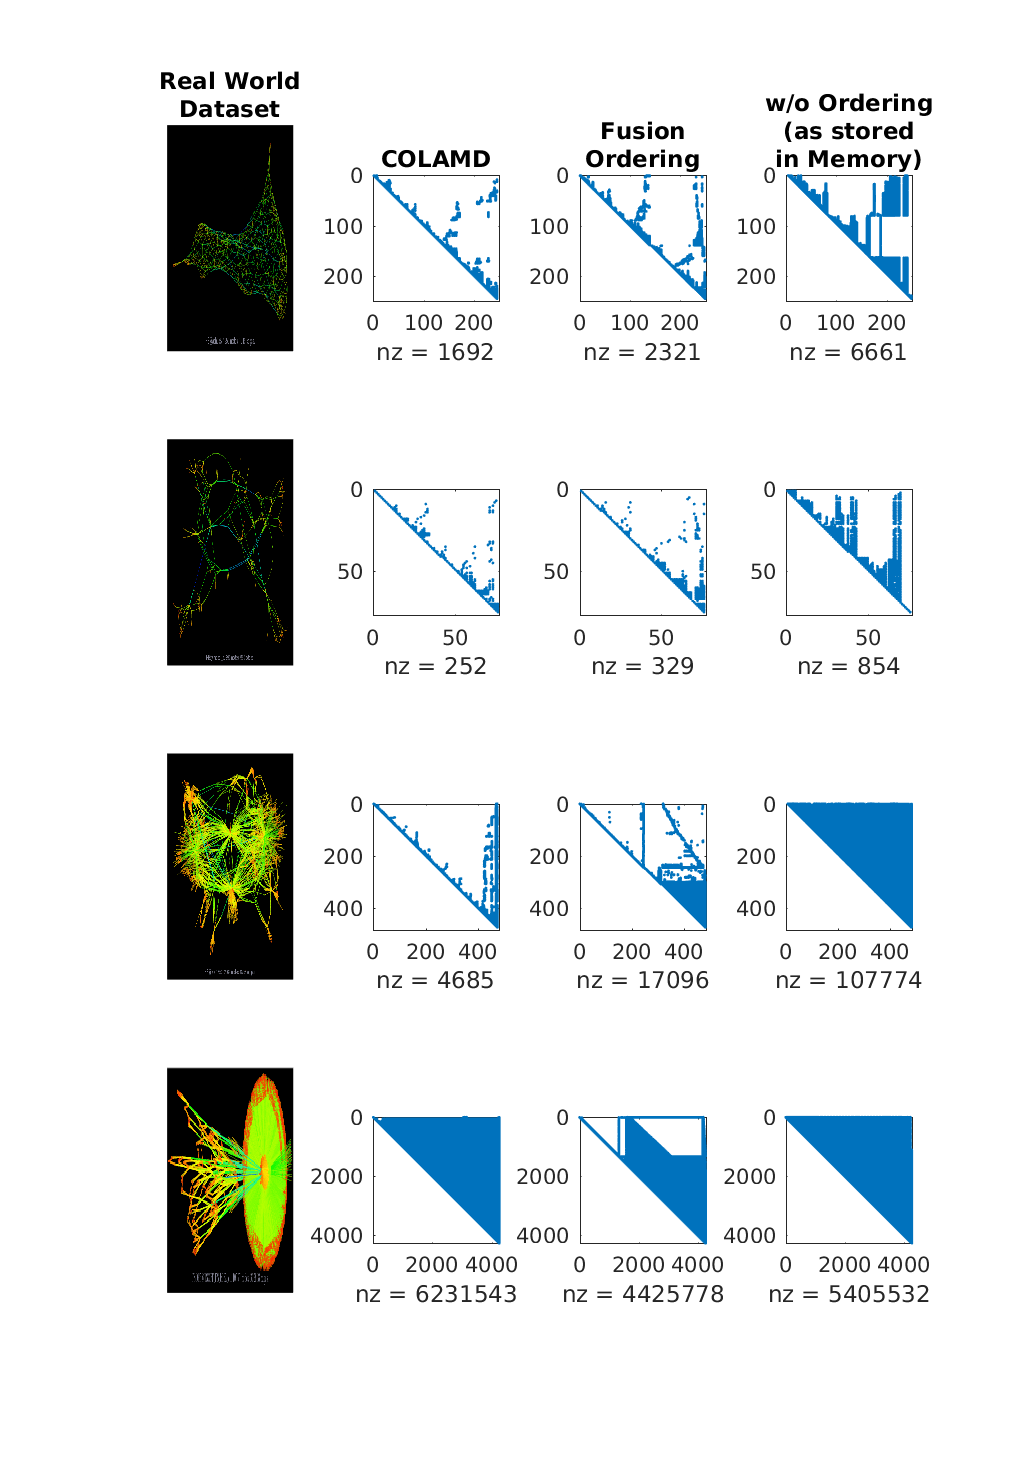
\includegraphics[width=\textwidth]{Chapters/figures3/ordering_comparison_2}
\caption{Comparison of number of non-zeros in the square root factor from QR factorization between the COLAMD ordering (second column), proposed ordering (third column) and the order in which the variables are retrieved (third column). The first column is the graph representation of the matrices in their lowest energy state \cite{suitesparse}.}
\label{fig:ordering_comparison_2}
\end{figure}
\paragraph{}
A comparison between the three types of orderings based on time taken to factorize the matrix after applying those ordering to the factor graph is performed in Figure \ref{fig:factorization_time}. As mentioned earlier, the orthonormal $Q$ matrix from QR decomposition is never explicitly formed in practice and hence the value of time is only that required to compute the square root factor $R$. Same experiment as before, comparing the number of non-zeros in the square root factor obtained from different ordering is also done on 120 real world matrices and plotted in Figure \ref{fig:nnz_comparison}. It can be seen that the proposed fusion ordering takes less time for factorization in many cases. This might be because the proposed ordering is inspired from variable ordering  by nested dissection and is compatible to parallel decomposition \cite{parallelqr}.
\begin{figure}[!]
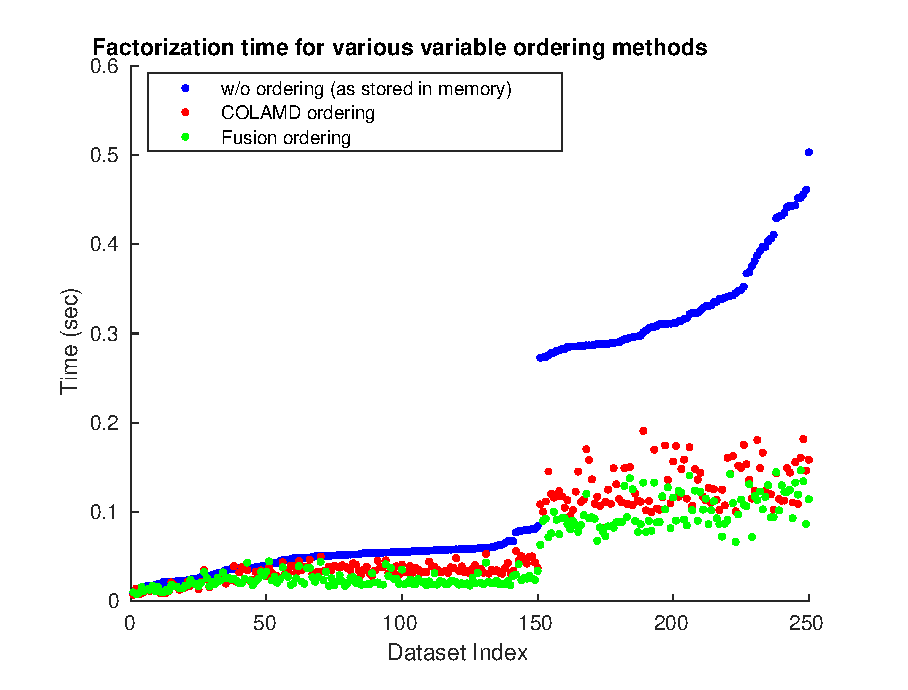
\includegraphics[width=\textwidth, height=0.4\textheight]{Chapters/figures3/factorization_time_comparison}
\caption{Comparison among different ordering schemes on the time taken to compute the square root factor $R$. It can be seen that the proposed fusion ordering takes less time than the COLAMD ordering as fusion ordering leaves the matrix in a state suitable for parallel QR decomposition \cite{parallelqr}.}
\label{fig:factorization_time}
\end{figure}
\begin{figure}[!]
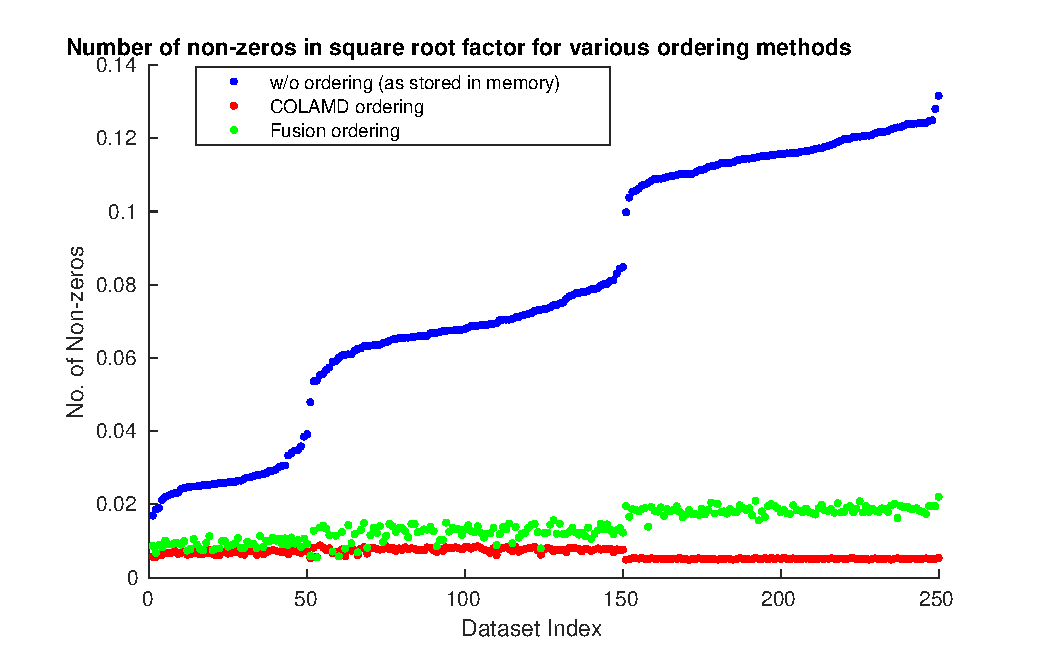
\includegraphics[width=\textwidth,  height=0.4\textheight]{Chapters/figures3/nnz_comparison}
\caption{Comparison among different ordering schemes on the number of non-zero fill-in produced. It can be seen that the COLAMD produces the least and is closely followed by fusion ordering. On the other hand, the variable memory order produces huge fill-in.}
\label{fig:nnz_comparison}
\end{figure}

%Relative ordering of c_affected 1 and c_affected 2 separately. c_2 affected is |c_1 affected| + argsort(c_2). Which sorted should be placed first out of two? The common elements placed at last.. Row ordering for stability... CFS like warranties?
%\newpage
%
%
%While combining the two graphs, \\
%Let $G^1 = (V^1, E^1)$ and $G^2 = (V^2, E^2)$ be the two graphs we are merging. Let $O^{G^1}$ and $O^{G^2}$ be their respective COLAMD orderings. Using these respective orderings the graphs $G^1$ and $G^2$ are stored as Bayes Tree. Let $C$ be the set of common nodes between the two graphs. Let $r_C^1$ and $r_C^2$ represent the set of nodes obtainedd from the Bayes Tree of $G^1$ and $G^2$ that gets affected on touching the common nodes $C$. The combined graph $G^C$ contains $V^C = C \cup r_C^1 \cup r_C^2$ and $E^C = E^p \cap (E^1 \cup E^2)$ where  $ E^p = \{ (v,w) \mid v \in V^C, w \in V^C, v \neq w\}$ is the power-set containing all the edges between nodes in $V^C$. \\
%
%\textbf{Relative Ordering:} As mentioned before, the ordering of the graph $G^1$ containing the vertices $V^1$ is given by $O^{G^1} = \{ o_1, o_2, ..., o_n \}$ where $n = \mid V^1\mid$. The relative ordering of the subgraph $S$ of the graph $G^1$ is given by 
%
%\begin{equation}
% O^S = arg sort(\bigcup_{v\in V^1} o^1(v))     
%\label{eq:relative}
%\end{equation}
%
%where $argsort$ gives the position of each element in the sorted array and $o^1(v)$ gives the order value of vertex $v \in V^1$ from the ordered set. $o^1(v)$ is equivalent to the value represented by $o$ with subscript $v$ in the set $O^1$. \\
%
%The combined graph ordering is done as follows - Let $O^{r_C^1}$, $O^{r_C^2}$ and $O^{C}$ be the relative ordering of $r_C^1$, $r_C^2$ and $C$ respectively. The relative ordering is calculated for $r_C^1$, $r_C^2$ and $C$ as shown in Eq. \ref{eq:relative} using their parent orderings $O^{G^1}$, $O^{G^2}$ and $O^{G^1}$ or $O^{G^2}$ respectively. This forms a block matrix as show in fig. \ref{fig:relative_colamd} that contains the nodes $r_C^1$, $r_C^2$ and $C$ in each of the blocks from left to right. The left top block contains the nodes in $r_C^1$ ordered using $O^{r_C^1}$, central bottom block contains $r_C^2$ ordered using $O^{r_C^2}$ and the right most block contains $C$ ordered using $O^C$. 
%
%\newpage
%
%Variable elimination [1, 4]
%originated in order to solve systems of linear equations, and was first applied in
%modern times by Gauss in the early 1800s [14]. [Related work]
%
%We also follow something like CCOLAMD to push the affected variable towards the end so as to reduce the computational steps in the upcoming updates. Tell this as though I did it. Put it as a part of HUND copy.
 % Experimental Setup

\chapter{Multi-robot Relative Pose Initialization}
\label{chap:four}

In this chapter, we address the problem of global consistency in the estimated values of the decision variables in least squares optimization \textit{across multiple robots.} The problem roughly boils down to initialization of the robot's relative pose in case of an encounter. Providing a good prior over the starting point of all robots that are consistent with respect to an external global frame partially solves the problem. However, it is a daunting task and also the presence of inter-robot constraints will further refine the estimates of the starting point of the robots. These inter-robot constraints are provided by introducing the ``global nail", that transforms the trajectory of any individual robot to global frame, as an estimation variable. By doing this, we demonstrate the alignment of map reconstructed by every robot based on the optimized trajectory. The next section briefly discusses the related work. Following that, we describe our proposed methodology. 

\section{Related Work}
Although the field of multi-robot SLAM has been explored significantly \cite{multi1, multi2, multi3, thrunmulti}, there is only a small body of work available on graph based multi-robot mapping. The problem of initialization of relative poses are addressed differently within various frameworks with qualifying assumptions. Early work in multi-robot mapping like \cite{multi3} assume known starting pose of all the robots with certainty in advance. A slight development in \cite{howardmulti} incorporates the initialization problem within the mapping framework but assumes that the very first encounter is perfect and hence neglects the subsequent encounters. It further developed into acknowledging the importance of initialization in \cite{thrunmulti} and consequently addressing it using the sparse extended information filter. In the context of smoothing and mapping (SAM), the most related work include cooperative SAM (C-SAM) \cite{csam}, tectonic SAM (T-SAM) \cite{tectonicsam} and multiple pose graph SLAM \cite{multipleisam}. Tectonic SAM is based on the similar principle that has the global nail to represent relative pose across different submaps of the region. It is batch algorithm for single robot. C-SAM is a batch algorithm for cooperative mapping and is tested only on simulation using two robots. Multiple pose graph SLAM is the one closest to our approach but does not explicitly consider the loop closures and landmarks while merging the pose graphs. 
 
\section{Relative Factor Graph Initialization} 
It is not necessary that all the robots in a multi-robot scenario start at the same location as assumed by several previous works. Figure \ref{fig:pose_graphs} shows the factor graph of three different robots. The factor graphs in this particular example can be considered to encode spatial information of the robot's trajectory and can be seen that they start at different positions and overlap. An arbitrary value as a prior factor over the starting pose works completely fine until a first direct encounter between the robots or indirect encounter by multiple robots visiting the same portion of the environment. The factor graph representation of a bunch of direct and indirect encounters is given in Figure \ref{fig:pose_graphs_encounter}. It is during this event that there is a conflict between the estimates of the state variables across different graphs and the measured local value of the encounter. This problem is resolved by introducing the ``global nail" for every individual robot's factor graph that converts the pose variable estimate locally consistent with the prior to the common global reference frame. Figure \ref{fig:pose_graphs_nails} introduces the global nails that constrain multiple robot trajectories using the relative transform from every robot frame to the common global frame. That said, the introduction of global nails might seem to remove the need for prior over the initial variables. Removing the prior does not affect the local measurements between variables but it will provide a gauge freedom for all the individual robot’s factor graphs. This is extremely problematic because the good linearization point can be far away from the variable estimates and any iterative optimization has the unintended consequence of getting stuck in the local minima. Thus the prior over the initial variables and the global nails are both essential to estimate the states of all the robots departing from various and uncertain starting locations. 
\begin{figure}
\centering
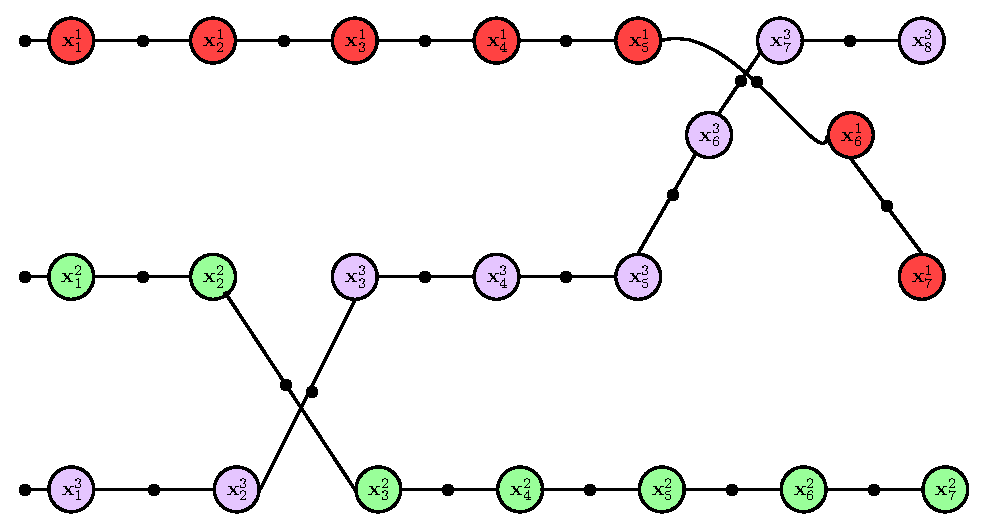
\includegraphics[width=\textwidth]{Chapters/figures4/pose_graph}
\caption{Factor graphs of three different robots. For this example, it can be considered that they also represent the spatial information of the trajectory.}
\label{fig:pose_graphs}
\end{figure}
\begin{figure}
\centering
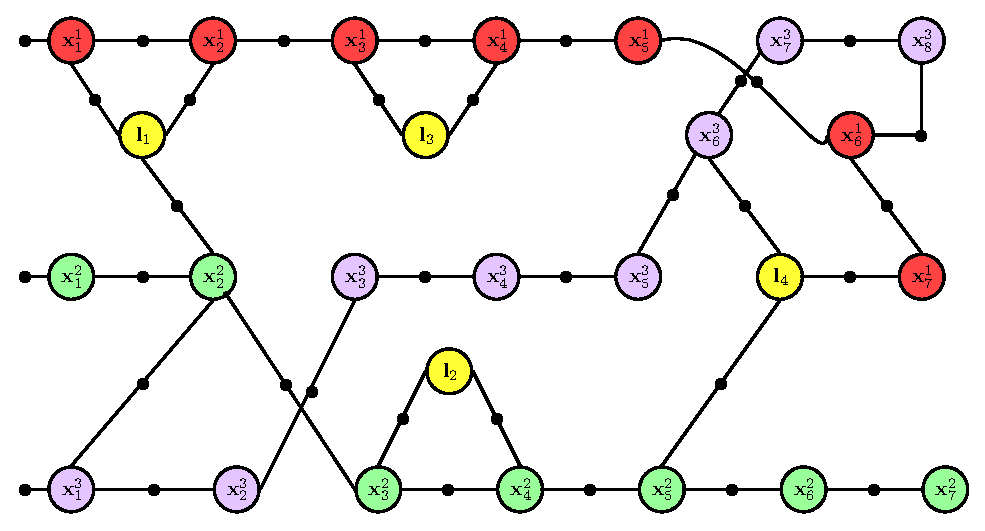
\includegraphics[width=\textwidth]{Chapters/figures4/pose_graph_encounters}
\caption{The set of direct and indirect encounters between robots in their overlapping trajectories are expressed. An indirect encounter is landmark connecting two different factor graphs and direct encounter is shown by a factor directly connecting two different factor graphs.}
\label{fig:pose_graphs_encounter}
\end{figure}
\begin{figure}
\centering
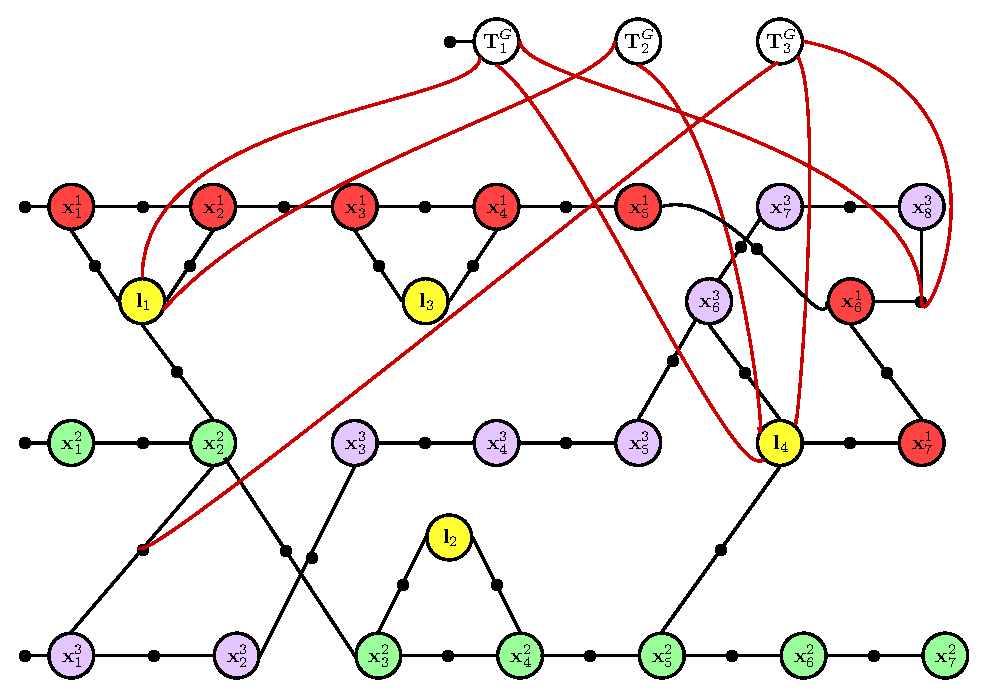
\includegraphics[width=\textwidth]{Chapters/figures4/pose_graph_with_nail}
\caption{The same encounters as in the previous figure but using the relative factor graph formulation. A global nail $T_r^G$ is introduced for each trajectory that specify the offset with respect to the global frame. All the encounters are connected with the global nail to account for multiple, uncertain encounters converging towards optimal solution over time.}
\label{fig:pose_graphs_nails}
\end{figure}
 
\paragraph{}
Using the global nail transforms the respective poses of each pose graph into a common global reference frame where the comparison becomes possible. This is illustrated using an example encounter in Figure \ref{fig:err_func}. The transform $T_G^1$ and $T_G^2$ are optimized such that the following equation representing the error on $l_1$ is as low as possible:
\begin{equation}
T_1^GT_{x_1^1}^1l_1^{x_1^1} - T_{2}^GT_{x_{2}^{2}}^{2}l_1^{x_{2}^{2}}
\label{eq:err_func_example}
\end{equation}
\begin{figure}[H]
\centering
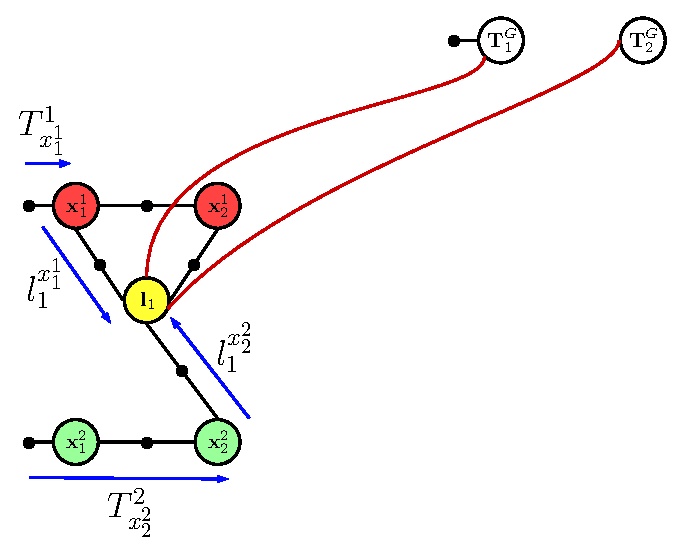
\includegraphics{Chapters/figures4/err_func}
\caption{Labelling the parts of a single encounter to understand the formulation of global nail factor.}
\label{fig:err_func}
\end{figure}
In the above Equation \ref{eq:err_func_example} the terms $l_1^{x_1^1}$ and $l_1^{x_{2}^{2}}$ are obtained from the sensor measurements like fiducial detection as explained in the next chapter. The terms $T_{x_1^1}^1$ and $T_{x_{2}^{2}}^{2}$ are the direct reflection of the value of prior over the initial variable of each factor graph and $T_1^G$ and $T_{2}^G$ are the variables to be estimated. The new type of factor that relates the encounter measurement along with the global nail is mathematically formulated as follows:
\begin{equation}
\sum_{n=1}^N \bigg\lvert\bigg\lvert T_r^GT_{x_i^r}^rl_n^{x_i^r} - T_{r^\prime}^GT_{x_{i^\prime}^{r^\prime}}^{r^\prime}l_n^{x_{i^\prime}^{r^\prime}}\bigg\rvert\bigg\rvert_{\Gamma_n}^2
\label{eq:err_func}
\end{equation}
where $r$ and $r^\prime$, $i$ and $i^\prime$ are the indices of robot and robot poses. $\Lambda_n$ denotes the corresponding direct or indirect encounter covariance. The above error function to be minimized is added to the least squares formulation in Equation \ref{eq:multilinlsopt} incrementally for every encounter. 
\paragraph{}
Now it should be noted that the overall system encompassing all the factor graphs faces gauge freedom. This is restricted by adding a prior over the first global nail. All the other global nails are added as they are needed. Generally, the covariance of the prior is made large because it is very likely to conflict when there is an encounter. The alignment of the maps and the improvement in the estimation quality is discussed and displayed in Chapter \ref{chap:six}.
 % Experiment 1

\chapter{Improved Viola-Jones Object Detection for Landmark Extraction}
\label{chap:five}

Viola-Jones object detection algorithm \cite{violajones} is a gold-standard in computer vision to detect trained objects at a very high speed using boosted classifiers. Because of their speed, they are used for object detection based landmark extraction in SLAM. In our multi-robot evaluation dataset, all the robots are fitted with a unique fiducial to represent their identity. Apart from this, the environment also contains fiducial markers that can be considered as landmarks in the map. In order to detect these with at a much lower false positive rate, at a lower resolution and eventually at a higher speed we improve the algorithm to utilize all the color channels in the input image. The original version works only on grayscale images. The key requirements for our scenario include high detection percentage with lower false positive rate and more importantly, the detection of the fiducial markers at various scale. As the robots are navigating, the target fiducial may come near or move away resulting in change in the size of fiducial on the captured image over continuous frames. The Haar features in Viola-Jones algorithm are perfectly suitable for this as they are scale invariant. We retain this property of the algorithm and increase the detection percentage along with the detection speed by leveraging the additional information obtained by using all the channels of the image. The improved version uses the same metric used in the original version to score a Haar feature but does it for all the channels of the input image. Thus the score is represented as a vector as opposed to a scalar value in the original version. These vectors are then ranked using linear discriminant analysis. We train a classifier to detect these fiducial markers using this improved version of Viola-Jones algorithm. The increase in the time complexity is matched by the ability to achieve better detection rates at lower resolution thereby producing a lower detection time overall. 
\paragraph{}
Since the detection algorithm and in general SLAM problem is very time sensitive, it is important to understand how the various tunable parameters affect the detection time. This chapter focuses on the complexity analysis of the multi-scale and multi-channel decision tree based detector. The algorithm learns a decision tree during the training stage which is usually evaluated on the test image set using a sliding window approach for multiple sizes of the window (scale invariance). In the next section, I would shed some light on few relevant works that have extended the original work of Viola-Jones in different contexts such as improving false alarm rate, modifications in Haar features, weighting schemes in Adaboost etc. There is no particular work that specifically deals with a detailed theoretical complexity analysis of the final detector although there has been empirical analysis both in the original paper \cite{violajones} and \cite{classifier4}. These theoretical results would be followed by a few experiments in the final section.

\section{Related Work}
In Viola-Jones object detection algorithm \cite{violajones}, the integral image for feature computation, Adaboost for feature selection and an attentional cascade for efficient computational resource allocation are the three key components behind achieving very high processing speed although the performance is same as the previous complex single stage classifiers. Following that, Lienhart \textit{et. al,} \cite{classifier4} did an empirical analysis of the original work and also introduced $45^{o}$ rotated HAAR features and verified that the Gentle Adaboost performs better than Real and Discrete Adaboost in terms of detection accuracy. A complete algorithmic description that explains the implementation logic behind Open Computer Vision library \cite{classifier14} is provided by \cite{classifier13}. Almost all the previously existing analysis deal only with the complexity of training the Cascade Classifier and just mention that the detection rate is very fast. To the best of my knowledge, this is the first analysis of the computational complexity of the Cascade Classifier object detection as a function of various tunable parameters.

\section{Theoretical Results}
The trained classifier performs a sliding window search over the target image for a fixed window size during every iteration. The set of tunable parameters for the Cascade Classifier Detector are:

\begin{itemize}
    \item The minimum window width and height of search, $W_{min}$ = $\{ w_{min}$, $h_{min} \}$
    \item The maximum window width and height of search, $W_{max}$ = $\{ w_{max}$, $h_{max} \}$
    \item The scale factor by which the window size grows from minimum to maximum, $\gamma_0$
    \item The minimum number of detections in the neighborhood to be selected as a true positive, $\beta$
\end{itemize}

\paragraph{}
The classifier is a cascaded set of decision trees and the number of such decision trees and the depth of each tree also influences the total time. However, since this value is constant for a given classifier it cannot be considered as a part of tunable parameters. Nevertheless, I have mentioned an upper bound on the number of evaluations of the entire decision tree over a given image. \\
\textbf{REMARK:} The classifier cannot detect target objects smaller than the trained window size. 

\subsection{Search window size and scale factor}
The maximum and minimum window sizes and the scale factor are interrelated and hence considered together for analysis. The size of the window along both the width and height is increased from the minimum to maximum value at the scale factor ratio. This is done to stick to the constant aspect ratio at which the classifier is trained. Let $w_t$ and $h_t$ be the training width and height. The set of all scale factor values is given by

\begin{equation}
\Gamma = \{ \gamma \mid w_t.\gamma \in [w_{min}, w_{max}] \cap h_t.\gamma \in [h_{min}, h_{max}], \gamma = \gamma_0, \gamma_0^2, ... ,\gamma_0^n\} \  \forall \ n \in \mathbb{N}     
\label{eq1}
\end{equation} 

%todo change "finer search window size."
where $\gamma_0$ is the initial value of scale factor which is also equal to the one input by the user. Generally, it is advised that $\gamma_0$ be in the positive neighborhood of 1, $\gamma_0 \rightarrow 1_+$ to get a finer search window size. The set of scale factors form a geometric progression with $\gamma_0$ being the common ratio between subsequent values. Now the set of image resolutions for which the integral image is to be calculated is given by 

\begin{equation}
I = \{ (x, y) | x = \frac{w_t}{r}, y = \frac{h_t}{r}\} \ \forall \ r \in \Gamma
\label{eq2}
\end{equation} 


\paragraph{}
The integral image is calculated for $\mid I \mid$ number of times. The number of elements in the set $I$ is actually the number of terms in the G.P represented by $\Gamma$ which can be calculated as follows.

\paragraph{}
Let $i$ denote the index of the terms in a G.P formed by initial value 1 and common ratio $\gamma_0$. Then the least and greatest value of $i$ that scales $w_t$ to the range $[w_{min}, w_{max}]$ are 

\begin{equation}
i^w_l = \left \lceil log_{\gamma_0} \left ( \frac{w_{min}}{w_t} \right ) \right \rceil
\label{eq3}
\end{equation}

\begin{equation}
i^w_g = \left \lfloor log_{\gamma_0} \left ( \frac{w_{max}}{w_t} \right ) \right \rfloor
\label{eq4}
\end{equation}

where the subscripts $l$ and $g$ represent the least and greatest index values respectively and $\lfloor.\rfloor$ and $\lceil.\rceil$ are the least and greatest integer functions.

\paragraph{}
Similarly, the least and greatest value of $i$ that scales $h_t$ to the range $[h_{min}, h_{max}]$ are 

\begin{equation}
i^h_l = \left \lceil log_{\gamma_0} \left ( \frac{h_{min}}{h_t} \right ) \right \rceil
\label{eq5}
\end{equation}

\begin{equation}
i^h_g = \left \lfloor log_{\gamma_0} \left ( \frac{h_{max}}{h_t} \right ) \right \rfloor
\label{eq6}
\end{equation}


\paragraph{}
To stick with the aspect ratio, only the terms that are common between the set of width and set of height ratios are considered. The number of common scale factors $K$ which is same as  $\mid \Gamma \mid$ and $\mid I \mid$ is in turn given by

\begin{equation}
K = \mid \Gamma \mid = \mid I \mid = min \{ i_g^w - i_l^w, i_g^h - i_l^h \}
\label{eq7}
\end{equation}

\begin{equation}
K = min \left \{ \left \lceil log_{\gamma_0} \left ( \frac{w_{max}}{w_{min}} \right ) \right \rceil , \left \lceil log_{\gamma_0} \left ( \frac{h_{max}}{h_{min}} \right ) \right \rceil \right \}
\label{eq8}
\end{equation}

Using the change of base rule,

\begin{equation}
K = min \left \{ \left \lceil \frac{ln \left ( \frac{w_{max}}{w_{min}} \right )}{ln\  \gamma_0}  \right \rceil , \left \lceil \frac{ln \left ( \frac{h_{max}}{h_{min}} \right )}{ln \ \gamma_0}  \right \rceil \right \}
\label{eq9}
\end{equation}


\paragraph{}
All example sub-windows used for training were variance normalized to minimize the effect of different lighting conditions. Normalization is therefore necessary during
detection as well. The variance of an image sub-window can be computed quickly using a pair of integral images. Recall that $\sigma^2 = m^2 - \frac{1}{N}\sum x^2$, where $\sigma$ is the standard deviation, $m$ is the mean, and $x$ is the pixel value within the sub-window. The mean of a sub-window can be computed using the integral image. The sum of squared pixels is computed using an integral image of the image squared (i.e. two integral images are used in the scanning process). During detection the effect of image normalization can be achieved by post-multiplying the feature values rather than pre-multiplying the pixels. Thus the integral image is calculated $2K$ number of times. The integral image is a summed area table data structure which is calculated  efficiently using a recursive algorithm. Though the computation of summed area table depends on the resolution of the image, the task of evaluating the intensities over any rectangular area requires only four array references. This allows for a constant calculation time that is independent of the size of the rectangular area. Also for multichannel images with $M$ channels, the number of integral image computations is $2MK$ times. This factor $M$ is the \textit{only} significant difference between multichannel cascade classifier detector and grayscale detector.

\subsection{Minimum number of neighbors}

The element set containing multiple detections of differently sized objects in target images are split into equivalency classes (clustering). We use a first order logic with a predicate that relates the objects in the set based on the test of similarity of rectangles. The running time of the clustering algorithm is actually \textit{independent} of the threshold $\beta$ that corresponds to the minimum number of neighbors jointly satisfying the predicate. The logic implements an $\mathcal{O}(N^2)$ algorithm for clustering a set of $N$ elements into one or more equivalency classes \cite{classifier1} as described using disjoint-set data structure representation \cite{classifier2}. For every element in the disjoint-set data structure of size $N^2$ the predicate is evaluated which returns either true or false. 
\paragraph{}
The predicate evaluates similarity of rectangles by taking any two elements from the input set along with the internal parameter $\epsilon$, $0 < \epsilon < 1$. \\

\setlength\parindent{24pt}
\textit{\textbf{Lemma:}}\textit{Two rectangles are similar if their sides are proportional.} 

\paragraph{}
This is checked by finding if all the sides of one rectangle is within $\Delta$ $=$ $\epsilon * (min(w_1, w_2),$ $min(h_1, h_2)) / 2$ of the other rectangle. \\
%todo formulate the necessity of a metric and why you need it. Then introduce delta

\setlength\parindent{24pt}
\textit{\textbf{Lemma:}}\textit{Two rectangles which are within a threshold $\Delta$ on all the four sides, for a $\Delta$ formulated using \textit{minimum} of width and height of the participating rectangles, are also within a threshold $\Delta$ for a $\Delta$ formulated using the maximum of their width and height.} 

\paragraph{}
Hence a $\Delta$ formed by the minimum of the their sides is a more restricted metric. The reason for formulating $\Delta$ is to account of uncertainty in similarity. The representative rectangle for all the equivalency class in the disjoint-set data structure is obtained by averaging all the constituent rectangles which is in turn returned as the detected rectangle. 

\subsection{Depth of the decision tree and target image resolution}

Though it looks like the detector is evaluated for various window sizes from minimum to maximum size, algorithmically the target image is shrunk from its original resolution to various sizes depending upon scale factors such that the objects of interest of sizes between minimum and maximum window size falls inside the constant window size. In other words, we are decreasing the size of the target image itself rather than increasing the size of the search window and rescaling the features appropriately. We take this rather long route of rescaling the image because the detection could be done using the same window size by which the classifier is trained. Although the values of the feature learned at every level of the classifier is normalized by the area of the feature, no clear explanation about guarantees on generality of learned classifier value for arbitrary rescaling of the feature considering linear interpolation of image and truncation/round-off errors in feature rescaling is given in the original paper \cite{violajones}. Obviously, by fractional rescaling the new correct positions become fractional. A plain vanilla solution is to round all relative look-up positions to the nearest integer position. However, performance may degrade significantly, since the ratio between the two areas of a feature may have changed significantly compared to the area ratio at training due to rounding. One solution is to correct the weights of the different rectangle sums so that the original area ratio between them for a given haar-like feature is the same as it was at the original size \cite{classifier4}. Nevertheless, by doing this reverse operation we end up linearly decimating the target image $\mid \Gamma \mid$ times and calculating integral image for each of them. From a memory perspective, the integral image for all the scales of the target image are computed and stored in a continuous serial buffer of size

$$ M \times \sum_{\gamma \in \Gamma} \left ( \frac{W}{\gamma} + 1 \right ) \left ( \frac{H}{\gamma} + 1  \right ) $$

where $W \times H$ is the resolution, $M$ is the number of channels of the target image and $\Gamma$ is the set of scale factors.

\paragraph{}
For a decision tree of $S$ stages and depth $d_s$ per stage where $s \in S$, an upper bound on the number of evaluations of all the stages of the decision tree is given by 

\begin{equation}
\le \sum_{\gamma \in \Gamma} \left \{ \left ( \frac{W}{\gamma} - w_t + 1 \right ) \left ( \frac{H}{\gamma} - h_t + 1  \right ) \times \sum_{s \in S} d_s \right \}
\label{eq10}
\end{equation}

where $W \times H$ is the resolution of the target image, $w_t \times h_t$ is the training resolution and $\Gamma$ is the set of all scale factors. 
\paragraph{}
\textbf{Note}: An implementation detail is that, for integral image resolutions whose corresponding scale factor is less than 2, the cascaded decision tree is only evaluated over every other pixel along width and height. Also, the entire continuous buffer of integral image across various resolutions is striped into memory chunks of size 

\begin{equation}
\delta_i = 32 \times \frac{H}{\gamma_i W} \  \ \forall \gamma_i \in \Gamma
\label{eq11}
\end{equation}


where $32$ is code specific. In total, there are $\sum_i \delta_i$ chunks which are processed in parallel using TBB multi-threading library.


\section{Experiments run}
% {\it Note: Describe in as much detail as possible the experiments that you
% set up and ran over this week. These could have been exploratory ones to
% understand an algorithm/tool/package/domain/dataset/programming model, etc.
% These could have been proof of concept experiments run on synthetic data or
% small samples. The experiments could have succeeded or failed. But for each
% of the experiments, you should write down clearly why you decided to run the
% experiment. What was the set up? All the parameters used, no. of runs, etc.
% Document all the outcomes clearly. Which parameter settings did the
% experiment succeed, when did it fail. Why did you choose a certain setting?
% Tabulate things clearly.. and where possible, draw graphs/charts etc.

% Clearly document your code as well. Keep around different versions, with
% comments describing what is different in each version. Try to follow some
% coding standards. In experiments that take a long time to run, save as much
% of the intermediate computation as possible. Do not write out only averages
% to the file. This might take slightly longer to run initially, but will save
% a lot of time when needing to re-run the experiments. For example, if you
% want to do some feature computation and then run a classifier on some data,
% save the computed features also. That way when you want to run a new
% classifier you don't have to compute features again.}
%"change ref in  span of a typically setup storeaisle shelf as shown in Fig.\ref"
The Haar Cascade Classifier \cite{violajones} described so far is used to detect the fiducial markers on top of every robot and in the environment in an online fashion. The biggest advantage of the Cascade Classifiers are their rapid speed of detection despite very long training time. The complexity analysis summarised in this report gives an idea on the sensitivity of each classifier parameter on the detection time. A conservative search size may detect all object instances but it is time critical to have a tight estimate that is just enough to detect all such instances.
\paragraph{}
From the theoretical results, it is clear how different values of the parameters are mathematically related. For this experiment we trained a fiducial marker with a training window size $63 \times 35$ using Gentle Adaboost \cite{classifier6,classifier7}.  In order to prove that the detection time is logarithmically related to the size of the search space defined by maximum and minimum window size, I ran the algorithm with multiple search search sizes decided by minimum and maximum window size. For the simplicity of understanding and denoting, the search size $\mathcal{S}$ can be represented as the length of line joining the right bottom corners of the minimum and maximum sized search rectangles.
\begin{equation}
\mathcal{S} = \sqrt{w_{max}^2 + h_{max}^2} - \sqrt{w_{min}^2 + h_{min}^2}
\label{eq12}
\end{equation}

\begin{figure}[h]
    \centering
    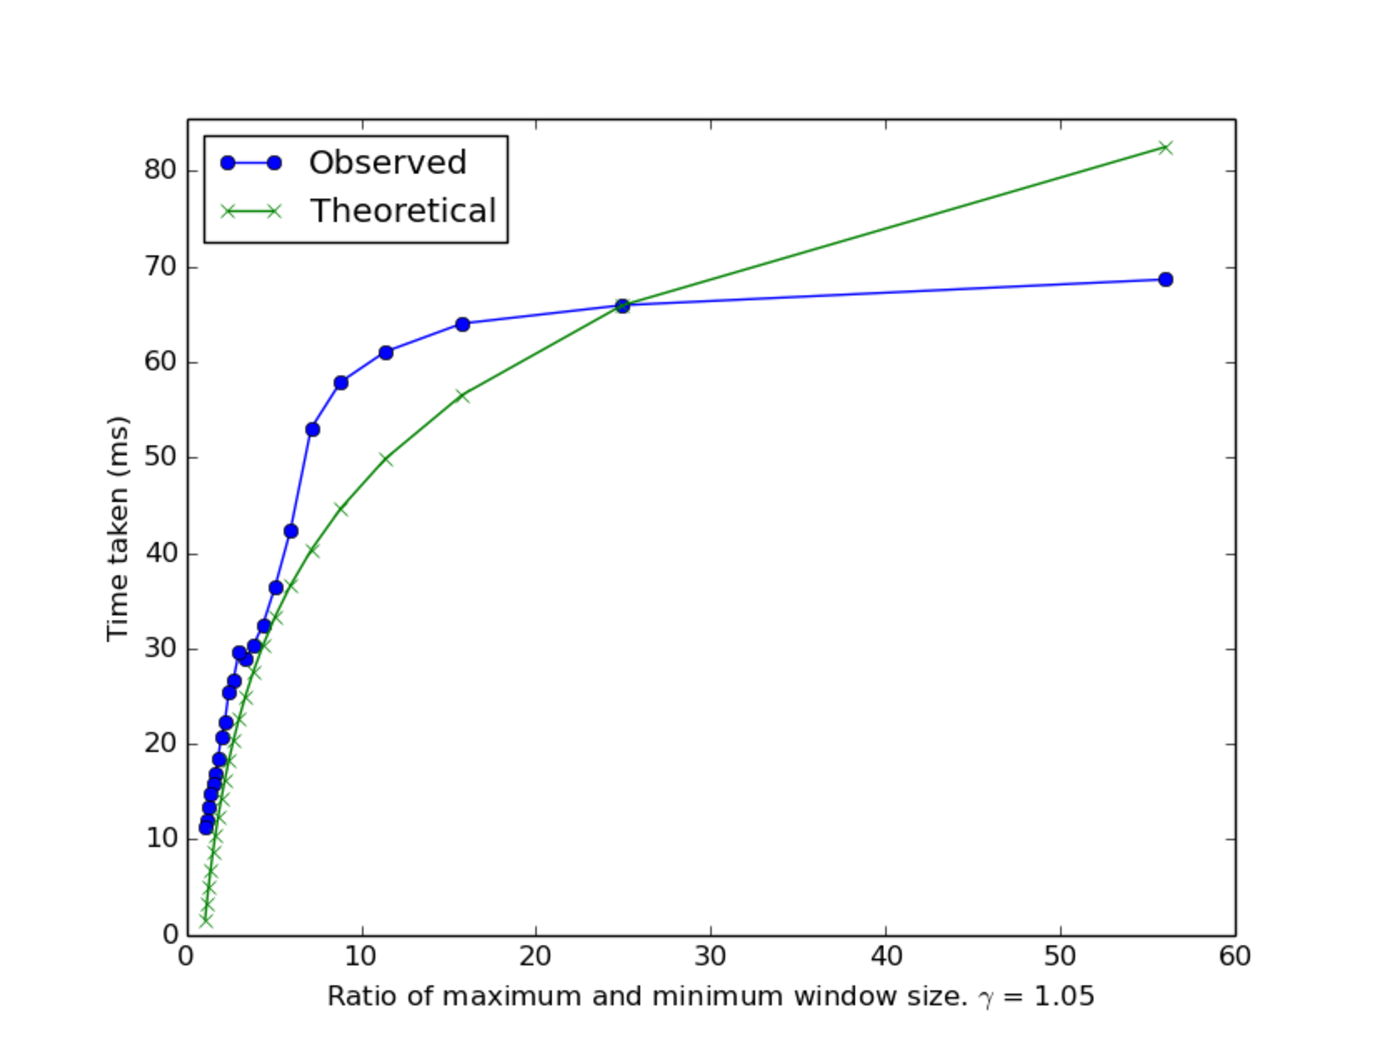
\includegraphics[width=\textwidth]{Appendices/figures1/winSize_vs_time}
    \caption{Comparison of ratio of maximum and minimum search window size with time taken taken for detection. It is clear from the shape of curve (blue) connecting the time taken for every search size that it varies logarithmically. The ideal curve (green) is just shown as a reference of a log curve and is not metrically accurate because we are trying to explain the theoretical complexity.}
    \label{one}
\end{figure}

\paragraph{}
The resolution of each source image captured by the camera that form the panorama is $1920 \times 2560$. But as mentioned before, because of the various aisle section depths and camera perspective the search rectangle size has to vary across the average size. The search size characterized by the ratio of maximum and minimum window size is started from $W_{min}=(480, 274)$, $W_{max}=(518, 296)$ and broadened till $W_{min}=(63, 35)$, $W_{max}=(980, 560)$. In every iteration, the gap between the minimum and maximum window size is reduced by a step size $s = 24$ pixels, $i.e$ the minimum height is increased by 12 pixels and maximum height is decreased by 12 pixels with their corresponding widths being aspect ratio adjusted. The final time of detection for a given search gap is found by averaging the detection time over 291 images having slightly varying target object size. Fig. $\ref{one}$ shows the various search size represented by the ratio of maximum and minimum window sizes plotted against the detection time(blue dots connected by a blue line). It can be seen from the shape of the curve that it approximates the logarithmic complexity. The green curve is the true log curve plotted with the ratio of maximum and minimum window size, $i.e. \ log_\gamma(\frac{W_{max}^i}{W_{min}^i})$. This experiment empirically verifies that the detection time scales logarithmically with the search size.

\paragraph{}
The second experiment is to empirically verify that the detection time varies \textit{inverse logarithmically} with the increase in the scale factor, which is the step size from the minimum to maximum window size of detection. The experiment was conducted with the constant minimum window size $W_{min}=(63, 35)$ and maximum window size $W_{max}=(980, 560)$. The scale factor, $\gamma$ is increased in steps of 0.02 starting from $\gamma = 1.01$. It can be seen from the plot in Fig. \ref{two} that the detection time decreases inverse logarithmically with the increase in scale factor as explained theoretically by Eqn. \ref{eq9}. The green curve in Fig. \ref{two} is the ideal curve that is plotted with the different scale factors and constant detection window size using the formula derived in Eqn. \ref{eq9}, $i.e. \ log_{\gamma_i}(\frac{W_{max}}{W_{min}})$.

\begin{figure}[h]
    \centering
    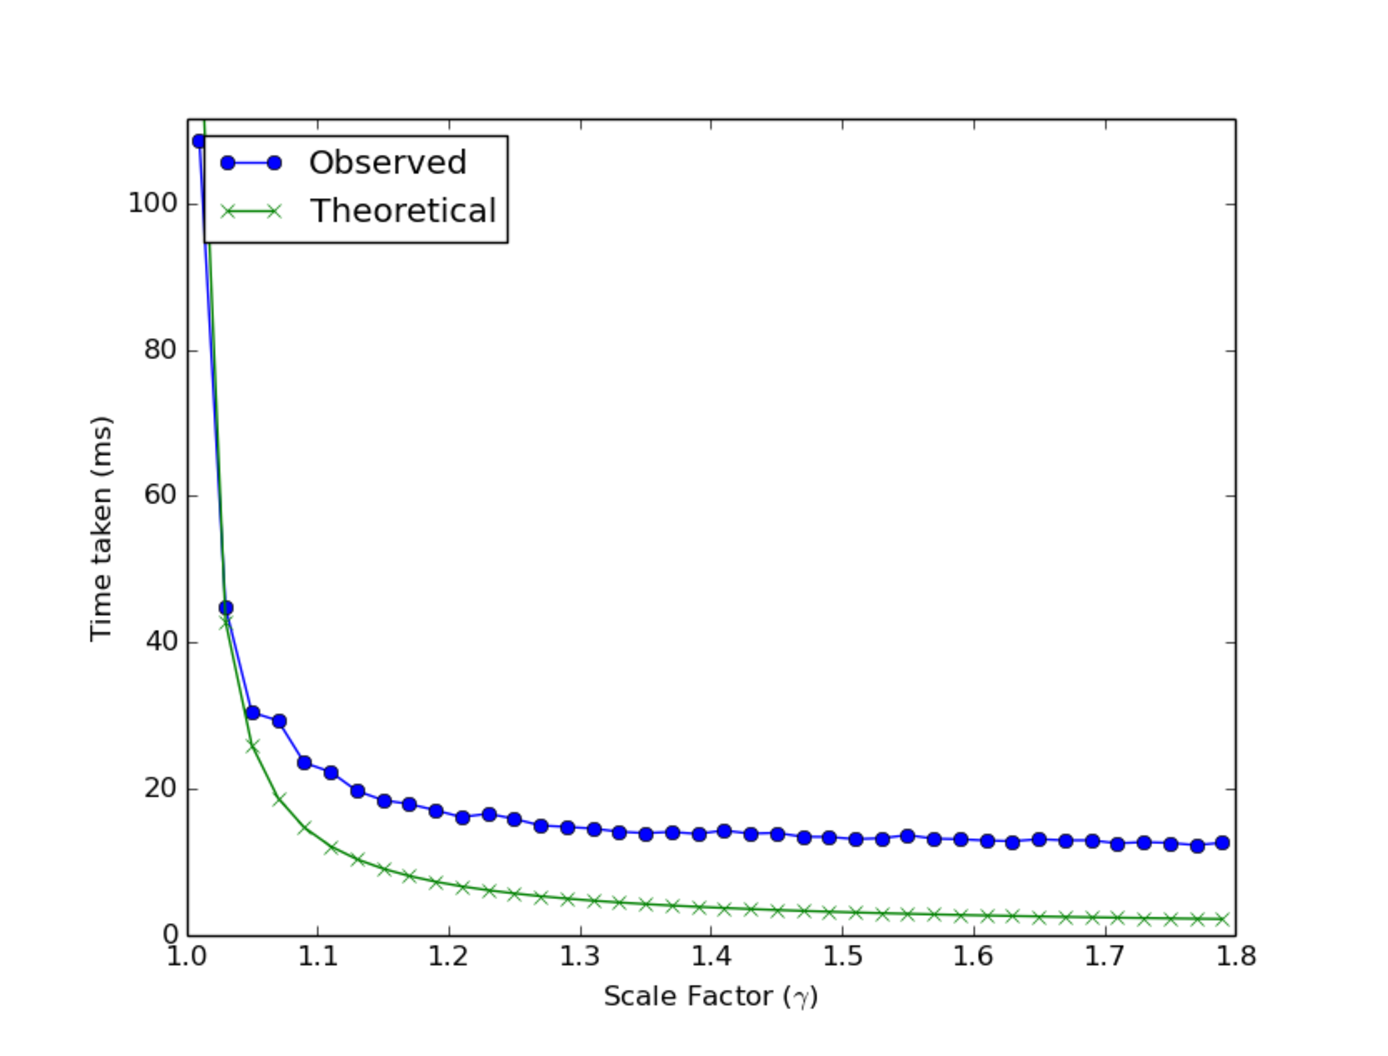
\includegraphics[width=\textwidth]{Appendices/figures1/gamma_vs_time}
    \caption{Comparison of scale factor with time taken taken for detection. It is clear from the shape of curve (blue) connecting the time taken for every scale factor that it varies \textit{inverse} logarithmically. The ideal curve (green) is just shown as a reference of a inverse log curve and is not metrically accurate because we are trying to explain the theoretical complexity.}
    \label{two}
\end{figure}
 % Experiment 2

\chapter{Results and Conclusions}
\label{chap:six}

In this chapter, we illustrate the performance of our fusion ordering in a real-world multi-robot dataset \cite{radish} recorded at AP hill, Virginia. For our datasets, we use a canonical scan-matcher \cite{csmicp} that remembers a short history of scans corresponding to the key frames, fits contours to the data, and for a new scan, finds a globally optimal alignment within a given search region. The canonical scan-matcher performs another least-squares optimization that requires an initial guess about the relative transform between the scans. The relative odometry measurement coming from the poses corresponding to those scans is used as an initial guess. Larger key frame sizes are also problematic as the scan ranges vary significantly due to seeing an altogether different structure of the environment. This leads to a large uncertainty in the estimate of the relative transform. It is also difficult to provide a good initial guess for large key frame sizes as the corresponding odometry transform is likely to be drifted. In our results, we project the raw laser scans from the optimized trajectory of every robot instead of occupancy grid as the occupancy grid can sometime hide the inaccuracies in the map, such as duplication of a wall. However, we also show the occupancy grid to comply with the usual practise in the SLAM literature.

\section{AP Hill Multi-robot Dataset}
The publicly available AP hill multi-robot dataset \cite{radish} is recorded using 4 mobile robots with significant overlap in their trajectories. The robots travel different paths covering different blocks in the building. Each robot is equipped with an odometer, a laser range finder, an inertial measurement unit and a camera. Encounter information is also provided along with the dataset. According to the dataset, all the robots start at nearly the same position, and hence the number of encounters in the later stages are less in number. In general, we increase the number of encounters by performing multi-channel fiducial detection (see Chapter \label{chap:five}) using the data obtained from the camera mounted on the robots. Getting a good map of the environment is an engineering task that requires tuning of several optimization parameters and those related to different measurement models. In this section, we will describe the numerical values that are used for different sensor models and ISAM2 algorithm in GTSAM optimizer \cite{gtsamhandson}. We will then present the timing analysis for using the fusion ordering for the combined graphs during every encounter. Finally the map alignment that is obtained by adding the relative transform between the trajectories as an estimation variable is displayed. 

\subsection{Tuning the Sensor Models and GTSAM Optimizer}
Getting the optimizer up and running to provide consistent and repeatable mapping results is generally preceded by developing accurate sensor models. The AP hill multi-robot dataset contains raw wheel encoder data, dead reckoning odometry data, laser range data, IMU data and the camera feed. The raw wheel encoder data is processed using a velocity motion model given in Appendix \ref{appendix:one}. The laser range data is used by the scan-matching module, also described in Appendix \ref{appendix:one}, to convert it into pose constraint. The IMU data is also treated in a similar manner to make it as a pose factor. Apart from the velocity model factors the dead reckoning odometry data is also used. Thus, all the pose variables are constrained by a minimum of four types of factors. In addition to the fiducials on top of every robot the environment also contains fiducials that serve as the landmarks. These fiducial and encounter information in the dataset are converted into a constraint between the poses and the landmarks/other robots. We also detect the same on the camera feed to further constrain the variables and over-determine the system. 
\paragraph{}
All these sensor models are accurate to a level that depends on the amount of uncertainty it introduces in the system. This level of uncertainty is captured by the covariance matrix that measures the joint variability of different random variables measured by the model. In other words, the sensor that is less accurate has a larger covariance. In many cases, they are provided by the sensor manufacturer. They can be used as a starting point and can then be tuned based on performance. For encoders like odometry, the error accrued is larger for larger sampling times. For such sensors, the covariance is tuned for unit time and scaled accordingly based on the time between different samples. In case of fiducial markers, the center of the detected fiducial is taken as the landmark position and therefore its covariance is also defined in terms of $x$, $y$ and $\theta$. The encounter covariance works same as the fiducial covariance as they are also fiducial markers attached to the robot. A loop closure introduces a correlation between the current pose and a previous pose occurred long back in time from which the current portion of the environment is observed. So a loop closure is also represented by a factor between robot poses at fairly farther time instants. The IMU model also estimates the relative transformation between robot poses and contains the same variables over which the covariance is represented. The tuned values of model covariance that are finally used for mapping are presented in Table \ref{table:cov}.
% Please add the following required packages to your document preamble:
% \usepackage{multirow}
% \usepackage{graphicx}
\begin{table}[]
\centering
\caption{Tuned covariance values of various sensor models used for mapping. These values are used to calculate the Bhattacharyya distance in the least-squares problem formulated in Chapter \ref{chap:two}. The covariance matrix for $n$ variables contain $n^2$ terms, but we tune the values only across the main diagonal (variance of each variable).}
\label{table:cov}
\resizebox{\textwidth}{!}{%
\begin{tabular}{|l|l|l|l|l|l|l|l|l|l|l|l|l|}
\hline
\multirow{2}{*}{Sensor Model} & \multicolumn{3}{l|}{robot 1} & \multicolumn{3}{l|}{robot 2} & \multicolumn{3}{l|}{robot 3} & \multicolumn{3}{l|}{robot 4} \\ \cline{2-13} 
                              & x (m) & y (m) & $\theta$ (rad) & x (m) & y (m) & $\theta$ (rad) & x (m) & y (m) & $\theta$ (rad) & x (m) & y (m) & $\theta$ (rad) \\ \hline
Velocity motion model         & 0.05  & 0.02  & 0.2          & 0.055 & 0.02  & 0.2          & 0.05  & 0.02  & 0.2          & 0.02  & 0.05  & 0.2          \\ \hline
Odometry model                & 0.04  & 0.02  & 0.5          & 0.04  & 0.03  & 0.5          & 0.05  & 0.022 & 0.1          & 0.023 & 0.013 & 0.2          \\ \hline
Landmark pose                 & 0.02  & 0.01  & 0.01         & 0.02  & 0.01  & 0.01         & 0.02  & 0.02  & 0.001        & 0.02  & 0.01  & 0.01         \\ \hline
IMU model                     & 0.02  & 0.01  & 0.05         & 0.02  & 0.01  & 0.05         & 0.01  & 0.01  & 0.001        & 0.01  & 0.01  & 0.01         \\ \hline
Loop closure factor           & 0.02  & 0.02  & 0.1          & 0.01  & 0.01  & 0.1          & 0.01  & 0.01  & 0.001        & 0.02  & 0.02  & 0.1          \\ \hline
Robot-robot encounter         & 0.01  & 0.01  & 0.2          & 0.01  & 0.01  & 0.02         & 0.01  & 0.01  & 0.2          & 0.01  & 0.01  & 0.2          \\ \hline
\end{tabular}%
}
\end{table}

\subsection{Global Map Alignment}
The global consistency in aligning the maps from multiple robots is achieved by using the ``global nails" introduced in Chapter \ref{chap:four}. The prior over the starting pose for the robots are initialized arbitrarily with minimum effort on tuning. Providing a prior over the starting pose is trivial for a single robot case as all the sensor measurements are locally consistent and the global alignment can be adjusted at any point in time. However, in a multi-robot scenario or in a lifelong and repeated mapping of the same environment, the prior over the initial pose should be known with certainty to fuse the common variables of estimation. To overcome this, an acceptable level of uncertain prior is tuned and improved via optimization with the global nail. The global nail corresponding to a particular robot is introduced only on its first encounter. A prior over the global nail of atleast one of the robots should be provided to prevent the entire system from having a gauge freedom. The alignment of the projected laser scan with and without using the global nail to calculate the relative transformation is shown in Figure \ref{fig:wo_align} and \ref{fig:w_align}. Each robot's trajectory is plotted with a unique color and its corresponding laser scan is depicted using a faded variant of the same color. The estimated final value of global nail variables are shown in the third column of the Table \ref{table:global_nail}. The second column lists the tuned values of all these variables and are used as an initial guess for optimization. The variable $T_r^G$ refers to the transformation from the starting point of robot $r$ to the global frame. 

\begin{table}[]
\centering
\caption{Tuned values for the prior over initial pose of every robot and the values obtained by optimization using the global nail.}
\label{table:global_nail}
\begin{tabular}{|l|l|l|l|l|l|l|}
\hline
\multirow{3}{*}{} & \multicolumn{6}{l|}{Value of relative pose graph transform} \\ \cline{2-7} 
 & \multicolumn{3}{l|}{w/o global nail} & \multicolumn{3}{l|}{w/ global nail} \\ \cline{2-7} 
 & x & y & $\theta$ & x & y & $\theta$ \\ \hline
$T_G^1$ & 0 & 0 & 0 & 0.401 & 0.299 & 0 \\ \hline
$T_G^2$ & -1.22 & 0.61 & 0 & -1.22 & 0.61 & 0 \\ \hline
$T_G^3$ & -2.44 & 0 & 0.1 & -2.44 & 0 & 0 \\ \hline
$T_G^4$ & -3.66 & 0.61 & 0 & -4.66 & 0.36 & 0 \\ \hline
\end{tabular}
\end{table}

\begin{figure}[H]
\centering
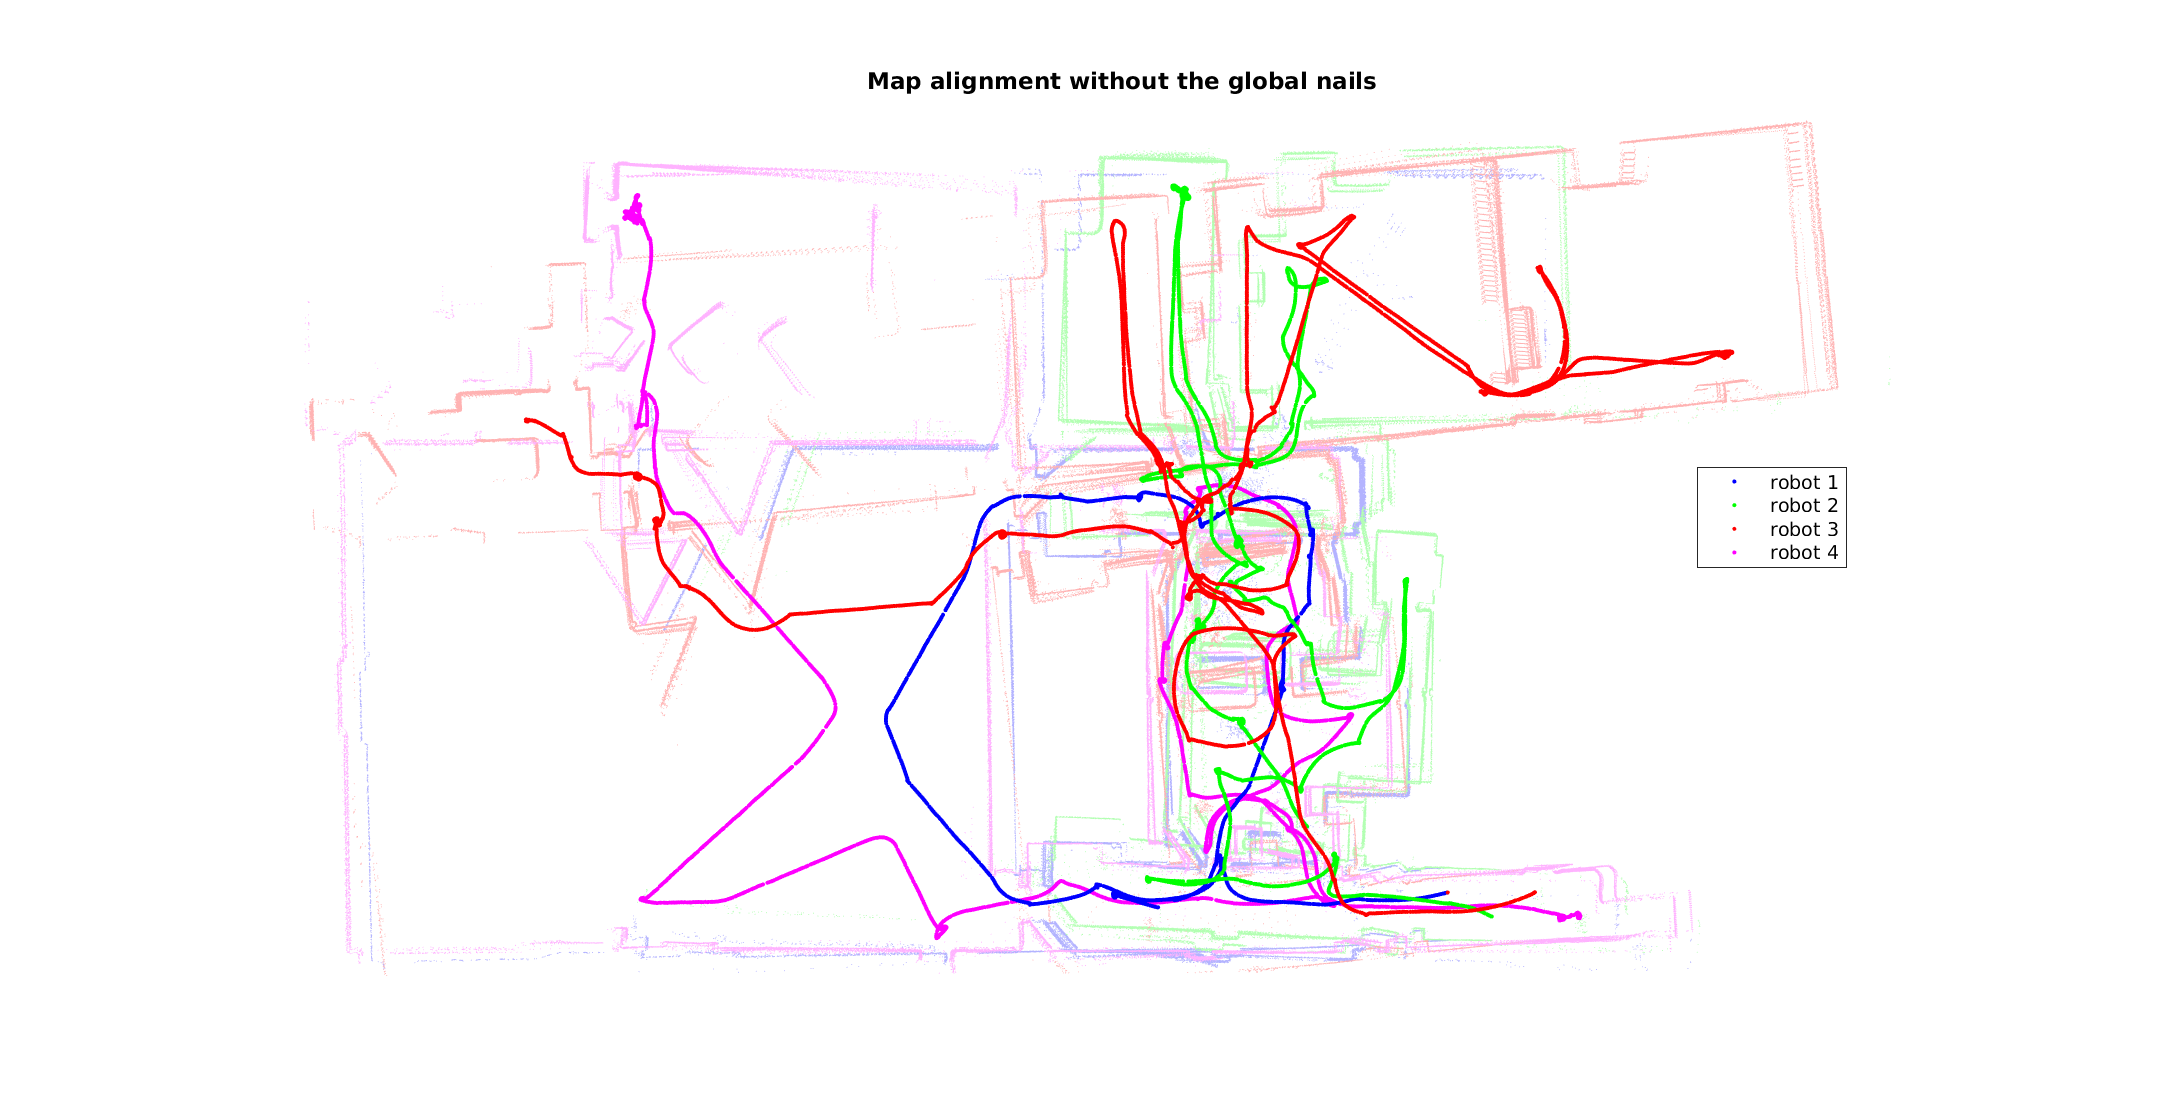
\includegraphics[width=\textwidth]{Chapters/figures6/without_map_alignment}
\caption{Overlay of laser scan projections from the smoothed trajectory of different robots. The optimization is done without the inter-robot relative pose transform constraint called ``global nail". It can be seen that, even after sufficient tuning of the prior over initial variables based on the map estimates at the early stages, we were not able achieve a total alignment.}
\label{fig:wo_align}
\end{figure}
\begin{figure}[H]
\centering
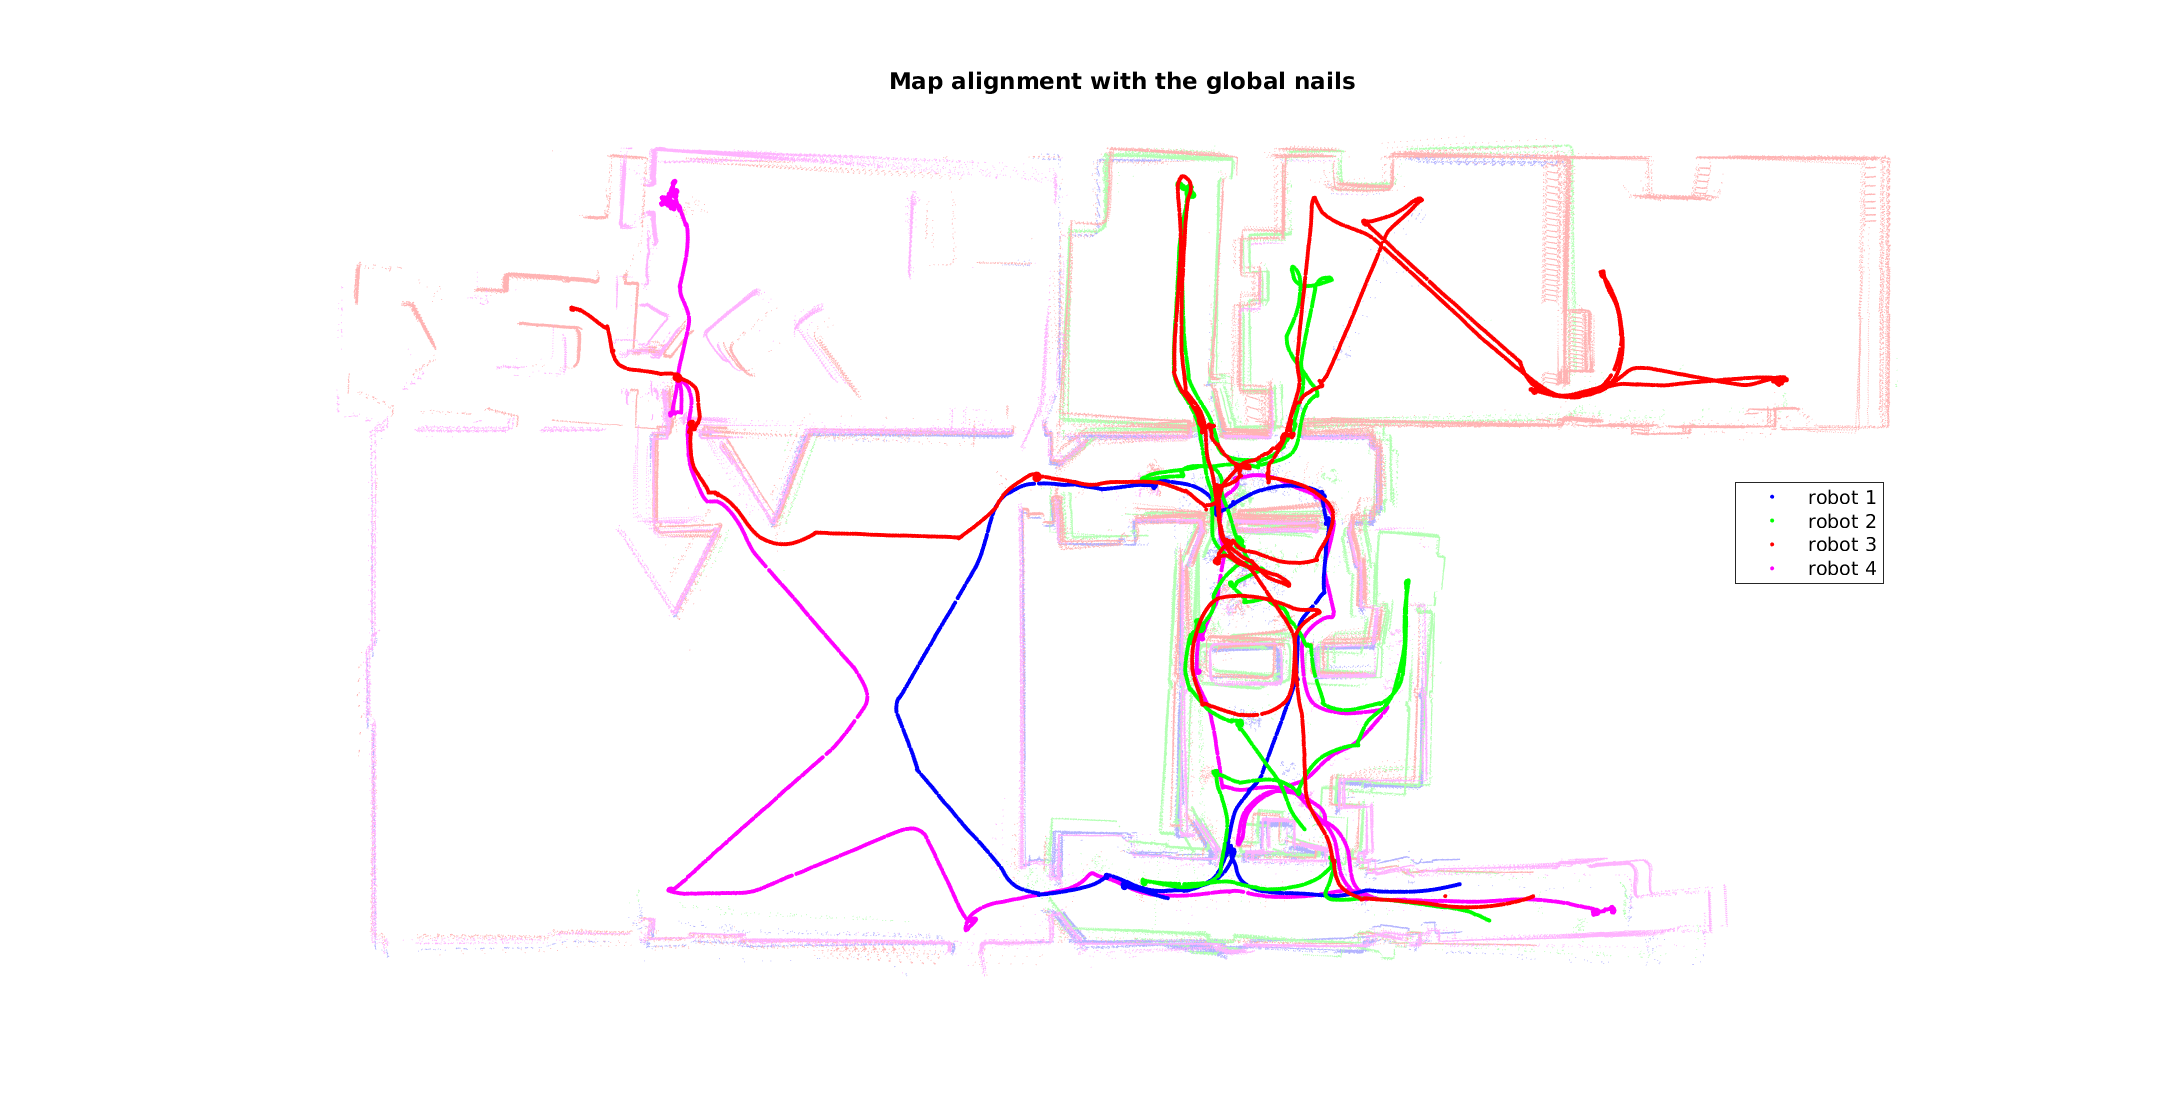
\includegraphics[width=\textwidth]{Chapters/figures6/with_map_alignment}
\caption{Overlay of laser scan projections from the smoothed trajectory of different robots. By adding the global nail constraints the relative transform between the robot trajectories are estimated accurates giving us a very good map alignment.}
\label{fig:w_align}
\end{figure}

\subsection{Fusion ordering vs. COLAMD ordering}
Whenever there is a direct or an indirect encounter, a factor between already existing common variable(s) or a new common variable is added. This leads to fusing the corresponding Bayes trees and marginalizing out the respective robot's variables. These marginals are then added as a strong prior to each robot's factor graph. The marginals of the ``global nail" variables from the fused graph are also added as a prior to the individual robot's factor graph that contains these ``global nail" variables. In practise, the graphs are fused for every few encounters and not every encounter. The performance is compared in terms of time it takes to calculate both these orderings. This ordering time does not include the time it takes to factorize the ordered measurement Jacobian. However, as fusion ordering leaves the Jacobian in a format explained in \cite{parallelqr} it can be subjected to parallel QR factorization. As a result, the time taken for factorization could be equal or lesser than using the COLAMD ordering. This phenomenon was already discussed while demonstrating the timing analysis on SuiteSparse dataset in Chapter \ref{chap:three}. 
\paragraph{}
The time taken for either of the ordering schemes are shown graphically using an encounter map in Figure \ref{fig:encounter_colamd} and \ref{fig:encounter_fusion}. The encounter maps contain the smoothed, centralized and final trajectory of all the robots using the combined information during every encounter. A line segment connecting the two trajectories indicate a robot-robot encounter from those poses at its endpoint. The color of the line segment reflects the time taken to compute the COLAMD ordering in Figure \ref{fig:encounter_colamd} or the fused ordering in Figure \ref{fig:encounter_fusion}. The color code reference is displayed with a color-bar on the right side of the encounter maps. The dataset contains roughly around 6000 direct robot-robot encounters and 300 indirect robot-landmark-robot encounters. It can clearly be observed that the color of the line segment for fusion ordering, when compared with that of nearly the same line segment for COLAMD ordering lies well below in the color-bar. This implies that the fusion ordering is faster in terms of computation than the COLAMD ordering. A more straightforward plot comparing the time taken by both these orderings is presented in Figure \ref{fig:fusion_vs_colamd}. Figure \ref{fig:fusion_vs_colamd} also includes the time taken for ordering the fused graph from indirect encounters.

\begin{figure}
\centering
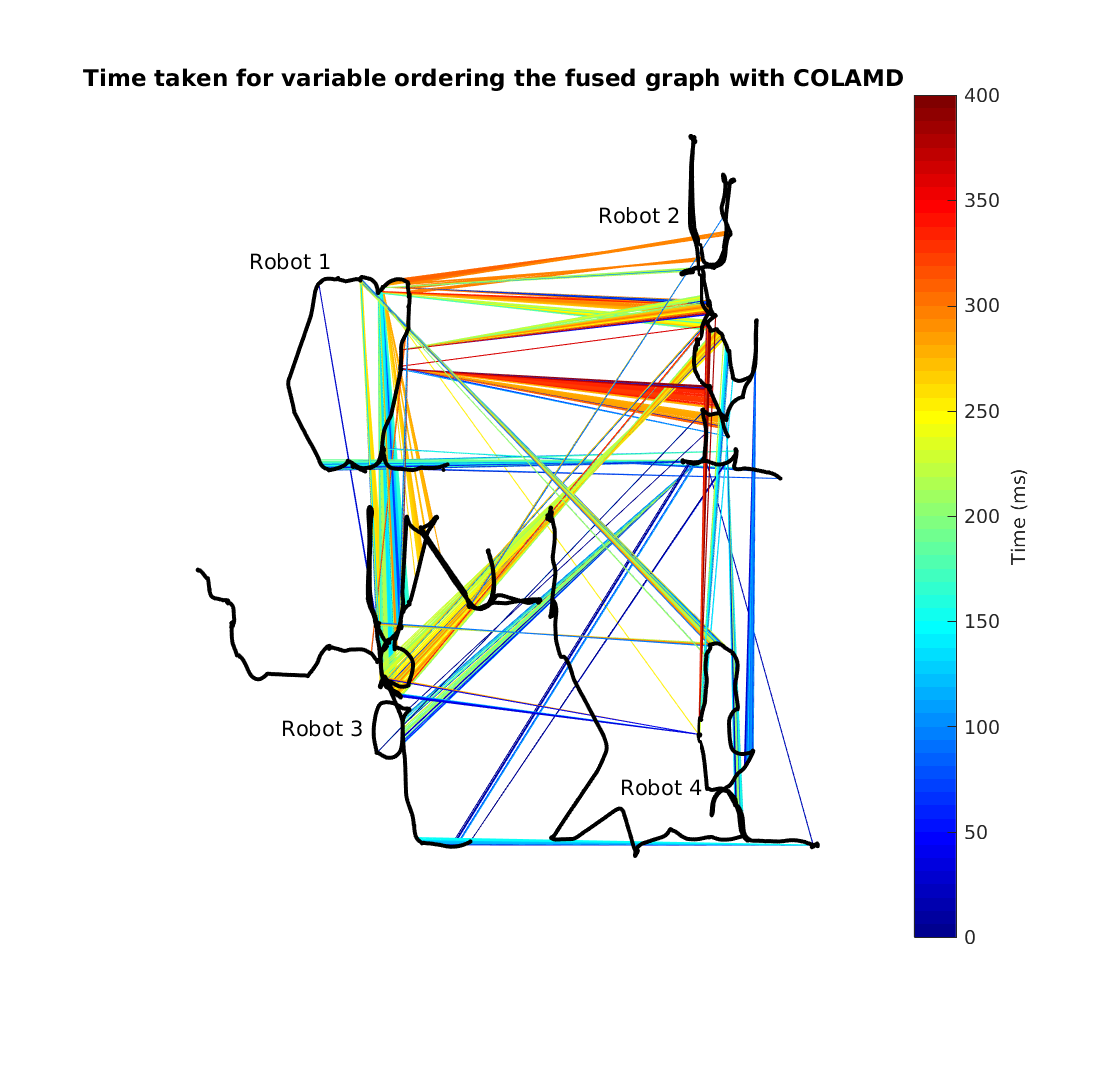
\includegraphics[width=\textwidth]{Chapters/figures6/colamd_ordering_encounter_colored}
\caption{The encounter map graphically describing the time taken for ordering the fused graph after every direct encounter using COLAMD \cite{colamd} ordering. The color of the line segment indicate the time taken and its endpoints indicate the poses corresponding to the encounter. A reference color bar is provided on the right. Note that the plot does not include indirect encounters as the trajectories are not in the original positioned and widely placed for clarity.}
\label{fig:encounter_colamd}
\end{figure}

\begin{figure}
\centering
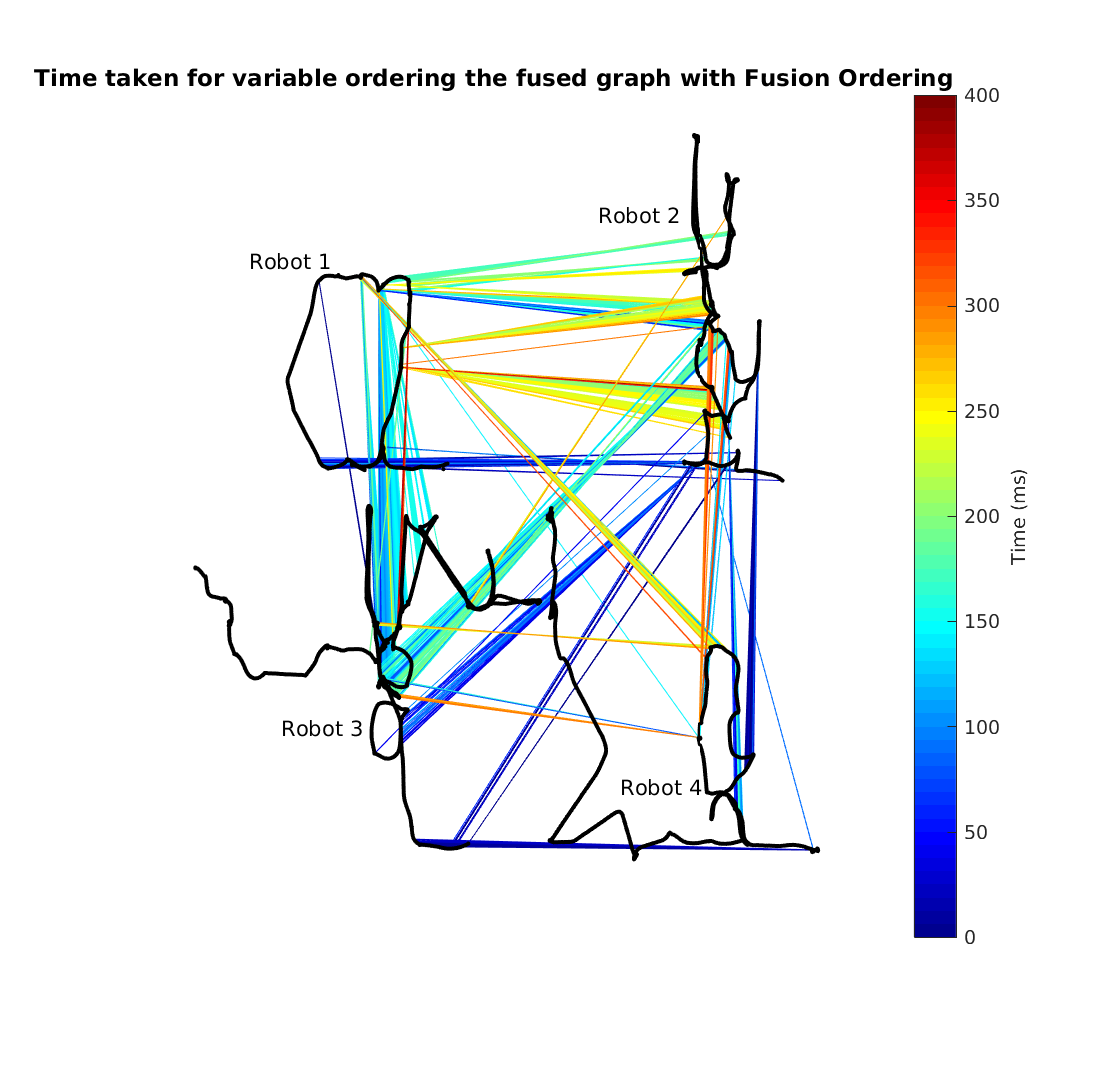
\includegraphics[width=\textwidth]{Chapters/figures6/fusion_ordering_encounter_colored}
\caption{The encounter map graphically describing the time taken for ordering the fused graph after every direct encounter using the proposed fusion ordering. The color of the line segment indicate the time taken and its endpoints indicate the poses corresponding to the encounter. A reference color bar is provided on the right. Note that the plot does not include indirect encounters as the trajectories are not in the original positioned and widely placed for clarity.}
\label{fig:encounter_fusion}
\end{figure}

\begin{figure}
\centering
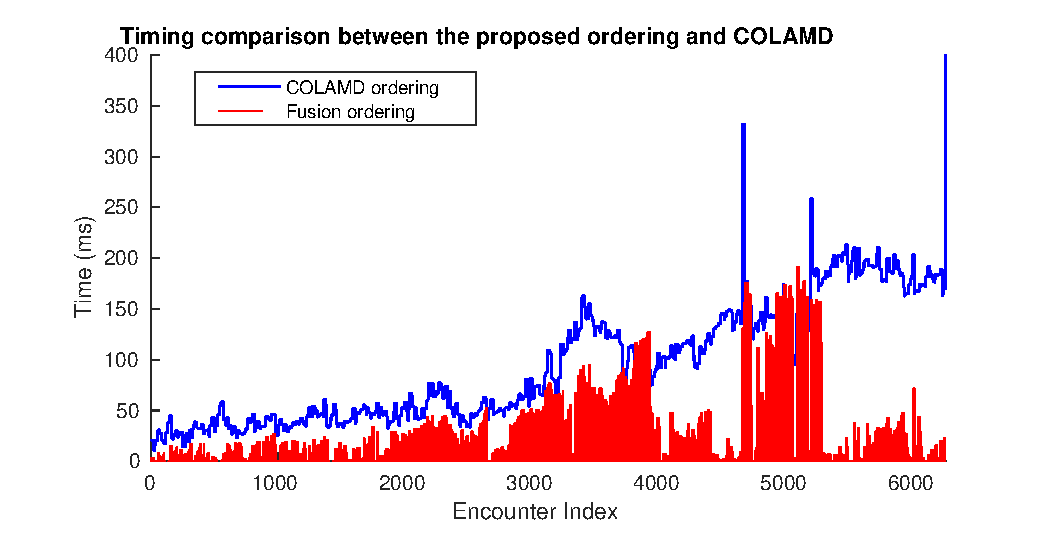
\includegraphics[width=\textwidth]{Chapters/figures6/time_fusion_vs_colamd}
\caption{Time comparison between the gold standard COLAMD and the proposed fusion ordering after every direct and indirect encounter. It can be observed that the time taken is lesser with fusion ordering for almost all the cases.}
\label{fig:fusion_vs_colamd}
\end{figure}

\section{Conclusions and Summary of Contributions}
In this thesis, we present a novel fusion ordering scheme for variable ordering the combination of multiple factor graphs using their parent ordering. We explain its relation with nested dissection to show the principle behind its working. A formal verification of the proposed algorithm is provided to ensure that it meets all the relevant standards and does not violate any canonical assumptions. One important aspect of the proposed algorithm is its potential to work in problems outside SLAM. Least squares is a standard approach for regression analysis and optimizing over-determined systems and is ubiquitous in engineering problems. Several factor graph applications in the field of finite element analysis, computational fluid dynamics and power network problem involve combining multiple graphs and variable ordering them for better estimation accuracy. We also presented a solution for relative pose graph initialization, a common problem in multi-robot mapping, that works within the framework of our problem formulation. The proposed factor type and the error function can be seamlessly added to the existing optimization problem and works for multiple and uncertain encounters with unknown data association. We demonstrate the results using standard real-world dataset from sparse linear algebra community called SuiteSparse and AP hill multi-robot dataset from radish repository. Introducing methods from the algebraic graph theory literature into the field of SLAM can be seen as another contribution. While several previous works have employed and innovated on matrix factorizations for SLAM, variable ordering the combined Jacobian from multiple robots has not been presented before. In particular, the combination of efficient fusion ordering, numerical stability ordering and relative pose graph initialization is novel and opens new possibilities that can be exploited in various robotics applications.

\section{Future Work}
Although the fusion ordering is quick and efficient in terms of time and storage, a thorough analysis about the change in the degree of the affected nodes in the fused graph with respect to the parent graph could be studied for different SLAM situations. This can lead to developing an upper bound on the additional number of non-zeros produced by using the fusion ordering instead of standard ordering techniques like COLAMD. Also, the structure of the ordered matrix coming out of fusion ordering is suitable for parallel QR decomposition according to \cite{parallelqr}, which I have not explored yet. The fusion ordering could be extended to work in the concurrent filtering and smoothing (CFS) framework \cite{cfs} for multiple robots. To get an end-to-end working real-time system it would interesting to investigate the bandwidth constraints in addition to the efficiency improvements proposed in this work. New factor types for encounters such as range-only or bearing-only might be studied in the context of relative pose graph initialization. 


 % Results and Discussion

%\input{Chapters/Chapter7} % Conclusion

%% ----------------------------------------------------------------
% Now begin the Appendices, including them as separate files

\addtocontents{toc}{\vspace{2em}} % Add a gap in the Contents, for aesthetics

\appendix % Cue to tell LaTeX that the following 'chapters' are Appendices

%\chapter{An Appendix}

Lorem ipsum dolor sit amet, consectetur adipiscing elit. Vivamus at pulvinar nisi. Phasellus hendrerit, diam placerat interdum iaculis, mauris justo cursus risus, in viverra purus eros at ligula. Ut metus justo, consequat a tristique posuere, laoreet nec nibh. Etiam et scelerisque mauris. Phasellus vel massa magna. Ut non neque id tortor pharetra bibendum vitae sit amet nisi. Duis nec quam quam, sed euismod justo. Pellentesque eu tellus vitae ante tempus malesuada. Nunc accumsan, quam in congue consequat, lectus lectus dapibus erat, id aliquet urna neque at massa. Nulla facilisi. Morbi ullamcorper eleifend posuere. Donec libero leo, faucibus nec bibendum at, mattis et urna. Proin consectetur, nunc ut imperdiet lobortis, magna neque tincidunt lectus, id iaculis nisi justo id nibh. Pellentesque vel sem in erat vulputate faucibus molestie ut lorem.

Quisque tristique urna in lorem laoreet at laoreet quam congue. Donec dolor turpis, blandit non imperdiet aliquet, blandit et felis. In lorem nisi, pretium sit amet vestibulum sed, tempus et sem. Proin non ante turpis. Nulla imperdiet fringilla convallis. Vivamus vel bibendum nisl. Pellentesque justo lectus, molestie vel luctus sed, lobortis in libero. Nulla facilisi. Aliquam erat volutpat. Suspendisse vitae nunc nunc. Sed aliquet est suscipit sapien rhoncus non adipiscing nibh consequat. Aliquam metus urna, faucibus eu vulputate non, luctus eu justo.

Donec urna leo, vulputate vitae porta eu, vehicula blandit libero. Phasellus eget massa et leo condimentum mollis. Nullam molestie, justo at pellentesque vulputate, sapien velit ornare diam, nec gravida lacus augue non diam. Integer mattis lacus id libero ultrices sit amet mollis neque molestie. Integer ut leo eget mi volutpat congue. Vivamus sodales, turpis id venenatis placerat, tellus purus adipiscing magna, eu aliquam nibh dolor id nibh. Pellentesque habitant morbi tristique senectus et netus et malesuada fames ac turpis egestas. Sed cursus convallis quam nec vehicula. Sed vulputate neque eget odio fringilla ac sodales urna feugiat.

Phasellus nisi quam, volutpat non ullamcorper eget, congue fringilla leo. Cras et erat et nibh placerat commodo id ornare est. Nulla facilisi. Aenean pulvinar scelerisque eros eget interdum. Nunc pulvinar magna ut felis varius in hendrerit dolor accumsan. Nunc pellentesque magna quis magna bibendum non laoreet erat tincidunt. Nulla facilisi.

Duis eget massa sem, gravida interdum ipsum. Nulla nunc nisl, hendrerit sit amet commodo vel, varius id tellus. Lorem ipsum dolor sit amet, consectetur adipiscing elit. Nunc ac dolor est. Suspendisse ultrices tincidunt metus eget accumsan. Nullam facilisis, justo vitae convallis sollicitudin, eros augue malesuada metus, nec sagittis diam nibh ut sapien. Duis blandit lectus vitae lorem aliquam nec euismod nisi volutpat. Vestibulum ornare dictum tortor, at faucibus justo tempor non. Nulla facilisi. Cras non massa nunc, eget euismod purus. Nunc metus ipsum, euismod a consectetur vel, hendrerit nec nunc.	% Appendix Title

\chapter{Sensor Models}
\label{appendix:one}

\section{Velocity Motion Model}

The following basic physics based velocity model assumes that the robot can be controlled through two velocities, rotational and translational. The model takes these velocities as the input and gives the current pose obtained by commanding the robot with those velocities from the  previous pose. The translational velocity at time $t$ is given by $v_t$, and the rotational velocity by $\omega_t$. We arbitrarily postulate that positive rotational velocities $\omega_t$ induce a counter-clockwise rotation (left turns). Positive translational velocities $v_t$ correspond to forward motion. In reality the robot motion is subjected to noise and hence the actual velocity differ from the commanded one. Thus the actual velocity can be obtained by adding a noise term:

\begin{equation}
\begin{bmatrix}
\hat{v} \\ \hat{w} 
\end{bmatrix} = 
\begin{bmatrix}
v \\ w
\end{bmatrix} + 
\begin{bmatrix}
\epsilon_v \\ \epsilon_w
\end{bmatrix}
\end{equation}
where $\epsilon_v$ and $\epsilon_w$ are zero mean random variable with finite variance. At every iteration the raw wheel encoder data in terms of translational and rotational velocity is used to find the relative transform from the previous pose $(x_{t-1}, y_{t-1}, \theta_{t-1})$ to the next pose $(x_{t}, y_{t}, \theta_{t})$. 
\begin{equation}
\begin{bmatrix}
x_t \\ y_t \\ \theta_t
\end{bmatrix} = 
\begin{bmatrix}
x_{t-1} \\ 
y_{t-1} \\
\theta_{t-1}
\end{bmatrix} + 
\begin{bmatrix}
-\frac{\hat{v}_{t-1}}{\hat{\omega}_{t-1}}sin \theta_{t-1} + \frac{\hat{v}_{t-1}}{\hat{\omega}_{t-1}}sin(\theta_{t-1} + \hat{\omega}_{t-1} \Delta t) \\ 
\frac{\hat{v}_{t-1}}{\hat{\omega}_{t-1}}cos \theta_{t-1} - \frac{\hat{v}_{t-1}}{\hat{\omega}_{t-1}}sin(\theta_{t-1} + \hat{\omega}_{t-1} \Delta t) \\ 
\hat{\omega}_{t-1} \Delta t + \hat{\gamma}\Delta t
\end{bmatrix}
\end{equation}
The above model describes the exact final location of a robot moving in a circular trajectory of radius $r = \frac{\hat{v}}{\hat{\omega}}$. However, in reality the motion is affected by control noise and the commanded circular trajectory is actually not circular. The circle constrains the final orientation which is fixed by adding an additional robot specific noise term $\hat{\gamma}$ on the final orientation in the above equation. 

\section{Iterative Closest Point based Scan Matching}

Let $X$ and $P$ represent two laser scan measurements measured closely in time. Let $k$ be the number of scan indices in the laser scan measurement:
\begin{equation}
X = \{ x_1, x_2, \ldots, x_k \}	
\end{equation}
\begin{equation}
P = \{ p_1, p_2, \ldots, p_k \}	
\end{equation}
The model takes two laser scan data as input and gives the relative transform between the poses from which those laser scans were measured as output. The problem is formulated as a least-squares optimization that finds the translation $t$ and rotation $R$ which minimizes the sum of squared error:
\begin{equation}
E(R,t) = \frac{1}{K_p} \sum_{i=1}^{K_p} \norm{x_i - Rp_i - t}^2
\end{equation}
where $x_i$ and $p_i$ are the corresponding points between two laser scans. Calculating the corresponding points is the most expensive stage of the ICP algorithm. If there is no uncertainty in calculating the corresponding points or if the corresponding points are given beforehand then the relative translation and rotation can be calculated in a closed form.
\paragraph{}
In our case, it is $approximately$ calculated by projecting the points according to the view point \cite{csmpaper}. As a start, the initial guess provided using the odometry model is used as the view point and then shifted till convergence. In projection based matching there are slightly bad alignments in each iteration but it is one to two orders of magnitude faster than the closest point. It also requires the point-to-line error metric. Using the point-to-line error metric the above vanilla iterative closest point formulation becomes:
\begin{equation}
\min_{q_{k+1}} \sum_i (n_i^T[x_i \bigoplus q_{k+1} - \Pi \{ \mathcal{S}^{ref}, x_i\bigoplus q_k \}])
\end{equation}
where $q_i$ is the robot's pose in the world frame, $x_i$ are the points in the first scan, $\Pi \{ \mathcal{S}^{ref}, .\}$ is the projection on the reference surface, $n_i$ is the normal to the surface and $\bigoplus$ is the notation introduced by Lu and Milios for pose composition \cite{lumiliosfirstgraphslam}.

 % Appendix Title

%\input{Appendices/AppendixC} % Appendix Title

\addtocontents{toc}{\vspace{2em}}  % Add a gap in the Contents, for aesthetics
\backmatter

%% ----------------------------------------------------------------
\label{Bibliography}
\lhead{\emph{Bibliography}}  % Change the left side page header to "Bibliography"
\bibliographystyle{unsrtnat}  % Use the "unsrtnat" BibTeX style for formatting the Bibliography
\bibliography{Bibliography}  % The references (bibliography) information are stored in the file named "Bibliography.bib"

\end{document}  % The End
%% ----------------------------------------------------------------
